% =====================================================================
%  Building a Modern Personal Agent Harness
%  Beamer deck with TikZ system diagrams.
%  Build:  make        (or: pdflatex personal_agent_harness.tex  x2)
% =====================================================================
\documentclass[aspectratio=169,10pt]{beamer}

\usepackage[T1]{fontenc}
\IfFileExists{lmodern.sty}{\usepackage{lmodern}}{}
\usepackage{booktabs}
\usepackage{tabularx}
\usepackage{array}
\usepackage{colortbl}
\usepackage{adjustbox}
\usepackage{listings}
\usepackage{tikz}
\usetikzlibrary{positioning,arrows.meta,shapes.geometric,shapes.misc,shapes.symbols,fit,backgrounds,calc}

% ---------------------------------------------------------------------
%  Palette
% ---------------------------------------------------------------------
\definecolor{ink}{RGB}{15,23,42}
\definecolor{accent}{RGB}{37,99,235}
\definecolor{teal}{RGB}{13,148,136}
\definecolor{amber}{RGB}{217,119,6}
\definecolor{violet}{RGB}{124,58,237}
\definecolor{rose}{RGB}{225,29,72}
\definecolor{leaf}{RGB}{22,163,74}
\definecolor{slate}{RGB}{71,85,105}
\definecolor{sky}{RGB}{2,132,199}

% ---------------------------------------------------------------------
%  Beamer look
% ---------------------------------------------------------------------
\setbeamersize{text margin left=0.6cm, text margin right=0.6cm}
\setbeamertemplate{navigation symbols}{}
\setbeamercolor{structure}{fg=accent}
\setbeamercolor{normal text}{fg=ink}
\setbeamercolor{frametitle}{fg=white,bg=ink}
\setbeamerfont{frametitle}{size=\large,series=\bfseries}
\setbeamertemplate{frametitle}{%
  \nointerlineskip
  \begin{beamercolorbox}[wd=\paperwidth,ht=0.95cm,dp=0.3cm,leftskip=0.6cm]{frametitle}%
    \usebeamerfont{frametitle}\insertframetitle
  \end{beamercolorbox}%
  \vspace{-0.05cm}{\color{accent}\rule{\paperwidth}{1.2pt}}%
}
\setbeamertemplate{footline}{%
  \hspace{0.6cm}{\tiny\color{slate}Personal Agent Harness \textbullet{} \insertsection}%
  \hfill{\tiny\color{slate}\insertframenumber/\inserttotalframenumber}\hspace{0.6cm}%
  \vspace{0.18cm}}
\setbeamertemplate{itemize items}[circle]
\setbeamertemplate{enumerate items}[default]
\setbeamerfont{itemize/enumerate subbody}{size=\scriptsize}
\setlength{\leftmargini}{1.1em}

\lstset{basicstyle=\ttfamily\tiny, keywordstyle=\color{accent}\bfseries,
  commentstyle=\color{slate}\itshape, stringstyle=\color{teal},
  language=Python, showstringspaces=false, columns=fullflexible,
  frame=single, rulecolor=\color{ink!20}, backgroundcolor=\color{ink!3},
  xleftmargin=2pt, framexleftmargin=2pt}

% ---------------------------------------------------------------------
%  TikZ styles
% ---------------------------------------------------------------------
\tikzset{
  >={Stealth[length=1.8mm]},
  bx/.style={draw=#1!70!black, fill=#1!10, rounded corners=2pt, align=center,
             font=\scriptsize, inner sep=2.5pt, minimum height=0.62cm, line width=0.6pt},
  bx/.default=accent,
  sbx/.style={bx=#1, font=\tiny, minimum height=0.45cm, inner sep=1.8pt},
  sbx/.default=accent,
  ar/.style={->, line width=0.7pt, draw=ink!65},
  dar/.style={<->, line width=0.7pt, draw=ink!65},
  dsh/.style={->, line width=0.6pt, draw=ink!55, dashed},
  lb/.style={font=\tiny, text=ink!80, fill=white, inner sep=1pt, align=center},
  nb/.style={font=\tiny, text=ink!80, inner sep=1pt, align=center},
  grp/.style={draw=#1!60!black, dashed, rounded corners=4pt, fill=#1!4, line width=0.5pt},
  grp/.default=slate,
  gl/.style={font=\tiny\bfseries, text=#1!65!black, anchor=south west, inner sep=1.5pt},
  gl/.default=slate,
  dia/.style={diamond, aspect=1.8, draw=#1!70!black, fill=#1!10, font=\tiny,
              inner sep=1pt, align=center, line width=0.6pt},
  dia/.default=amber,
}

% group box behind a set of nodes, with a label above its top-left corner
\newcommand{\group}[4]{% #1 name, #2 colour, #3 fit list, #4 label
  \begin{scope}[on background layer]
    \node[grp=#2, fit=#3, inner sep=5pt] (#1) {};
  \end{scope}
  \node[gl=#2] at (#1.north west) {#4};}

% rating dots (0..3), more = better
\newcommand{\rate}[1]{%
  \foreach \i in {1,2,3}{\ifnum\i>#1{\color{ink!20}\scalebox{1.6}{$\bullet$}}\else{\color{accent}\scalebox{1.6}{$\bullet$}}\fi}}

\newcommand{\pill}[2]{\tikz[baseline=(p.base)]\node[fill=#1!15,text=#1!70!black,rounded corners=2pt,
  inner sep=1.5pt,font=\tiny\bfseries](p){#2};}

\newenvironment{diagram}{\begin{adjustbox}{max width=\linewidth, max totalheight=0.80\textheight, center}}{\end{adjustbox}}

% variant card: #1 title, #2 tikz body, #3 how, #4 best for, #5 watch out
\newcommand{\variant}[5]{%
  \begin{minipage}[t]{0.485\linewidth}
    {\small\bfseries\color{accent}#1}\par\vspace{2pt}
    \begin{adjustbox}{width=\linewidth, max totalheight=2.9cm, center}
    \begin{tikzpicture}#2\end{tikzpicture}
    \end{adjustbox}\par\vspace{3pt}
    {\scriptsize
    \textbf{How:} #3\par\vspace{1.5pt}
    \textbf{\color{leaf!70!black}Best for:} #4\par\vspace{1.5pt}
    \textbf{\color{rose!80!black}Watch out:} #5\par}
  \end{minipage}}

\title{Building a Modern Personal Agent Harness}
\date{September 2026}

% =====================================================================
\begin{document}

% ---------------------------------------------------------------------
\begin{frame}[plain]
\begin{tikzpicture}[remember picture, overlay]
  \fill[ink] (current page.south west) rectangle (current page.north east);
  \fill[accent] ([yshift=-3.2cm]current page.north west) rectangle ++(\paperwidth,0.08);
  \node[anchor=north west, text=white, font=\huge\bfseries, align=left, text width=14cm]
    at ([xshift=0.9cm,yshift=-1.1cm]current page.north west)
    {Building a Modern\\Personal Agent Harness};
  \node[anchor=north west, text=white!80!accent, font=\normalsize, align=left, text width=14cm]
    at ([xshift=0.9cm,yshift=-3.6cm]current page.north west)
    {Memory \textbullet{} browsing the internet \textbullet{} shopping \textbullet{} travel booking
     \textbullet{} negotiating late returns};
  \node[anchor=north west, text=white!70, font=\small, align=left, text width=14cm]
    at ([xshift=0.9cm,yshift=-4.5cm]current page.north west)
    {System diagrams, 14 architecture variants, a prototype stack for thousands of users,\\
     and the path to millions.};
  % little motif
  \foreach \x/\c/\t in {0/accent/Memory,1/teal/Tools,2/amber/Policy,3/violet/Durable,4/rose/Evals}{
    \node[draw=\c!60, fill=\c!75, text=white, rounded corners=2pt, font=\scriptsize\bfseries,
          minimum width=2.2cm, minimum height=0.6cm]
      at ([xshift=2.0cm+\x*2.55cm, yshift=1.3cm]current page.south west) {\t};}
  \node[anchor=south east, text=white!55, font=\scriptsize]
    at ([xshift=-0.6cm,yshift=0.3cm]current page.south east) {September 2026};
\end{tikzpicture}
\end{frame}

% ---------------------------------------------------------------------
\begin{frame}{Agenda}
\begin{columns}[T]
\column{0.5\textwidth}
\begin{enumerate}
  \item What a personal agent must do
  \item Reference architecture
    \begin{itemize}\item agent loop, memory, tools, browser, safety, payments\end{itemize}
  \item Use-case flows
    \begin{itemize}\item shopping, travel, negotiating a late return\end{itemize}
  \item 14 architecture variants + comparison
\end{enumerate}
\column{0.5\textwidth}
\begin{enumerate}\setcounter{enumi}{4}
  \item Prototype: 0 $\rightarrow$ thousands of users
    \begin{itemize}\item full technical stack, code sketch, 12-week plan, cost\end{itemize}
  \item Scaling to millions of users
    \begin{itemize}\item capacity math, cell architecture, cost-down, reliability, security, evals\end{itemize}
  \item Team, risks, takeaways
\end{enumerate}
\end{columns}
\vfill
{\scriptsize\color{slate} Vendor and protocol names are examples of each category as of Sept 2026; costs are order-of-magnitude
estimates at list prices -- validate before committing.}
\end{frame}

% =====================================================================
\section{Foundations}
% =====================================================================
\begin{frame}{What a personal agent must do}
\scriptsize
\renewcommand{\arraystretch}{1.35}
\begin{tabularx}{\linewidth}{>{\bfseries\raggedright\arraybackslash}p{2.2cm} X X X}
\toprule
Job & Example request & Hard parts & Capabilities needed\\
\midrule
Research \& browse & ``Best stroller for city + jogging, under \$600'' & untrusted web content, freshness, SEO spam & search, fetch, browser, citations, preference memory\\
Shopping & ``Reorder my usual coffee from the cheapest reliable seller'' & checkout flows, stock, fraud, payment & commerce APIs, browser checkout, virtual cards, order tracking\\
Travel & ``NYC$\rightarrow$Lisbon Oct 12--19, aisle, under \$900, use miles if better'' & volatile fares, holds, loyalty, rebooking & flight/hotel APIs, calendar, price watch, durable timers\\
Negotiation \& service & ``Return these boots -- it's day 35 of a 30-day window'' & persuasion within ethics, multi-channel, days of waiting & email, chat, voice, policy reasoning, follow-ups\\
Life admin & ``Cancel the gym, dispute this charge, renew my passport'' & identity, forms, 2FA, legal nuance & form filling, document vault, human hand-off\\
\bottomrule
\end{tabularx}
\end{frame}

\begin{frame}{Design principles}
\begin{columns}[T]
\column{0.5\textwidth}
\small
\begin{enumerate}
  \item \textbf{Durable by default} -- a return dispute lives for weeks; every step is checkpointed and resumable.
  \item \textbf{Memory is the product} -- sizes, seats, loyalty numbers, merchants you trust, what worked last time.
  \item \textbf{API first, browser second, human last} -- use the most reliable channel that covers the task.
  \item \textbf{Least privilege + explicit consent} -- scoped tokens, per-task spend caps, approval on anything irreversible.
\end{enumerate}
\column{0.5\textwidth}
\small
\begin{enumerate}\setcounter{enumi}{4}
  \item \textbf{Untrusted content is data, never instructions} -- web pages, emails and merchant chats cannot steer the agent.
  \item \textbf{Observable \& replayable} -- traces, screenshots, audit log for every action.
  \item \textbf{Cost-aware} -- model routing, prompt caching, compile repeated flows into scripts.
  \item \textbf{Honest agent} -- discloses it is an AI acting for a user; never misstates facts while negotiating.
\end{enumerate}
\end{columns}
\end{frame}

% =====================================================================
\section{Reference architecture}
% =====================================================================
\begin{frame}{Reference architecture}
\begin{diagram}
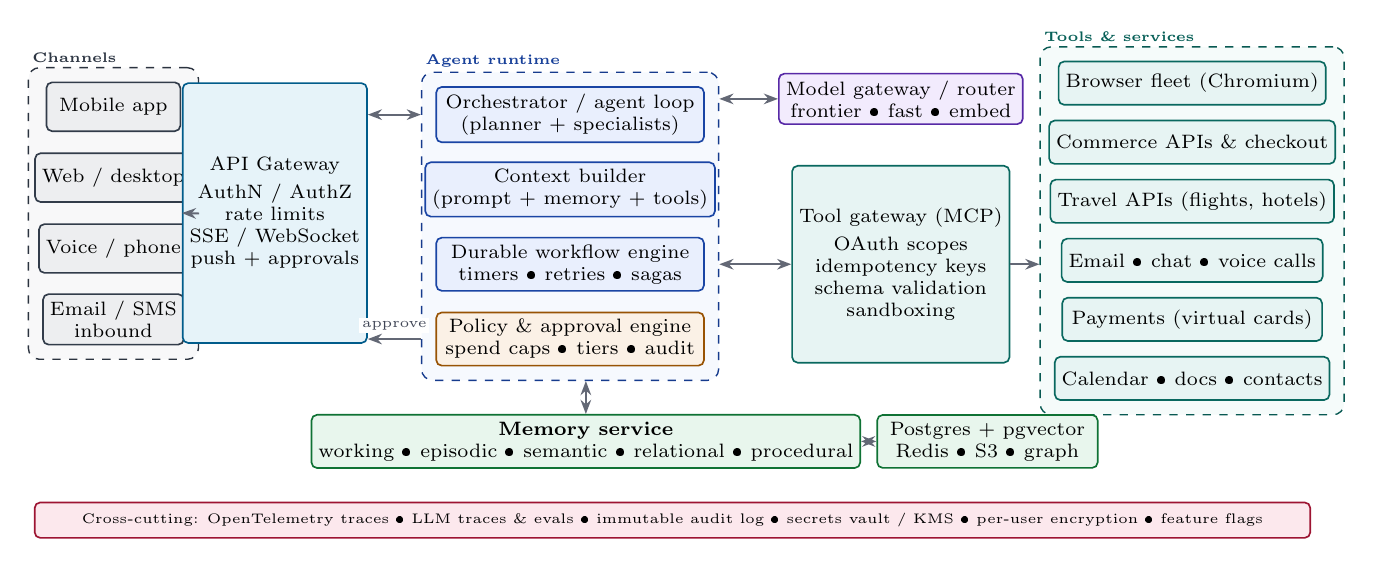
\begin{tikzpicture}
  % channels
  \node[bx=slate, minimum width=1.7cm] (mob) at (0.9,5.2) {Mobile app};
  \node[bx=slate, minimum width=1.7cm] (web) at (0.9,4.3) {Web / desktop};
  \node[bx=slate, minimum width=1.7cm] (voice) at (0.9,3.4) {Voice / phone};
  \node[bx=slate, minimum width=1.7cm] (inb) at (0.9,2.5) {Email / SMS\\inbound};
  \group{gch}{slate}{(mob)(inb)}{Channels}
  % gateway
  \node[bx=sky, minimum width=1.7cm, minimum height=3.3cm] (gw) at (2.95,3.85)
     {API Gateway\\[2pt]AuthN / AuthZ\\rate limits\\SSE / WebSocket\\push + approvals};
  % runtime
  \node[bx=accent, minimum width=3.4cm] (orch) at (6.7,5.1) {Orchestrator / agent loop\\(planner + specialists)};
  \node[bx=accent, minimum width=3.4cm] (ctx) at (6.7,4.15) {Context builder\\(prompt + memory + tools)};
  \node[bx=accent, minimum width=3.4cm] (dur) at (6.7,3.2) {Durable workflow engine\\timers \textbullet{} retries \textbullet{} sagas};
  \node[bx=amber, minimum width=3.4cm] (pol) at (6.7,2.25) {Policy \& approval engine\\spend caps \textbullet{} tiers \textbullet{} audit};
  \group{grt}{accent}{(orch)(pol)}{Agent runtime}
  % model gateway
  \node[bx=violet, minimum width=2.7cm] (mg) at (10.9,5.3) {Model gateway / router\\frontier \textbullet{} fast \textbullet{} embed};
  % tool gateway
  \node[bx=teal, minimum width=2.7cm, minimum height=2.5cm] (tg) at (10.9,3.2)
     {Tool gateway (MCP)\\[2pt]OAuth scopes\\idempotency keys\\schema validation\\sandboxing};
  % tools
  \foreach \n/\t/\y in {t1/Browser fleet (Chromium)/5.5, t2/Commerce APIs \& checkout/4.75, t3/{Travel APIs (flights, hotels)}/4.0,
                         t4/Email \textbullet{} chat \textbullet{} voice calls/3.25, t5/Payments (virtual cards)/2.5, t6/Calendar \textbullet{} docs \textbullet{} contacts/1.75}
     {\node[bx=teal, minimum width=3.3cm, minimum height=0.55cm] (\n) at (14.6,\y) {\t};}
  \group{gtools}{teal}{(t1)(t6)}{Tools \& services}
  % memory
  \node[bx=leaf, minimum width=5.4cm] (mem) at (6.9,0.95)
    {\textbf{Memory service}\\working \textbullet{} episodic \textbullet{} semantic \textbullet{} relational \textbullet{} procedural};
  \node[bx=leaf, minimum width=2.8cm] (store) at (12.0,0.95) {Postgres + pgvector\\Redis \textbullet{} S3 \textbullet{} graph};
  % cross-cutting
  \node[bx=rose, minimum width=16.2cm, minimum height=0.45cm, font=\tiny] (x) at (8.0,-0.05)
    {Cross-cutting: OpenTelemetry traces \textbullet{} LLM traces \& evals \textbullet{} immutable audit log \textbullet{}
     secrets vault / KMS \textbullet{} per-user encryption \textbullet{} feature flags};
  % arrows
  \draw[ar] (gch.east) -- (gw.west);
  \draw[dar] (gw.east |- orch) -- (grt.west |- orch);
  \draw[ar] (grt.west |- pol) -- node[lb, above=2pt]{approve} (gw.east |- pol);
  \draw[dar] (grt.east |- mg) -- (mg.west);
  \draw[dar] (grt.east |- dur) -- (tg.west |- dur);
  \draw[ar] (tg.east) -- (gtools.west |- tg.east);
  \draw[dar] (grt.south -| mem) -- (mem.north);
  \draw[dar] (mem.east) -- (store.west);
\end{tikzpicture}
\end{diagram}
\end{frame}

% ---------------------------------------------------------------------
\begin{frame}{The agent loop}
\begin{columns}[c]
\column{0.47\textwidth}
\begin{diagram}
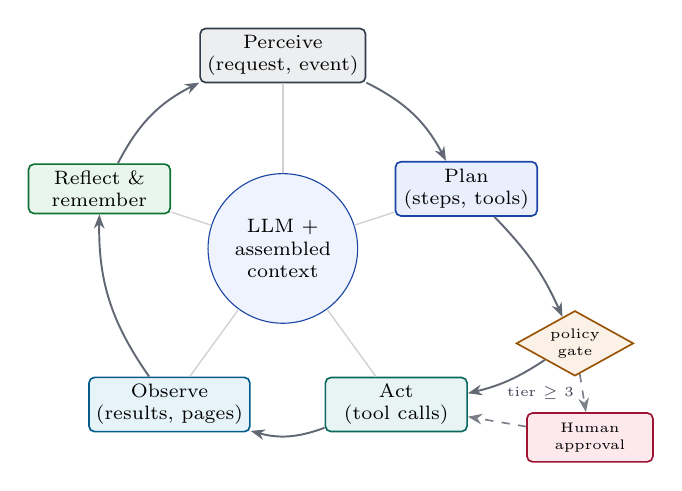
\begin{tikzpicture}
  \node[circle, draw=accent!70!black, fill=accent!8, font=\scriptsize, align=center, minimum size=1.9cm] (c)
     at (0,0) {LLM +\\assembled\\context};
  \foreach \n/\a/\t/\col in {pe/90/{Perceive\\(request, event)}/slate, pl/18/{Plan\\(steps, tools)}/accent,
      ac/-54/Act\\(tool calls)/teal, ob/-126/{Observe\\(results, pages)}/sky, re/162/Reflect \&\\remember/leaf}
    {\node[bx=\col, minimum width=1.8cm] (\n) at (\a:2.45) {\t};}
  \draw[ar] (pe) to[bend left=18] (pl);
  \node[dia=amber] (g) at (-18:3.9) {policy\\gate};
  \draw[ar] (pl) to[bend left=10] (g);
  \draw[ar] (g) to[bend left=10] (ac);
  \draw[ar] (ac) to[bend left=18] (ob);
  \draw[ar] (ob) to[bend left=18] (re);
  \draw[ar] (re) to[bend left=18] (pe);
  \node[bx=rose, font=\tiny, minimum width=1.6cm] (h) at (3.9,-2.4) {Human\\approval};
  \draw[dsh] (g) -- node[nb, left=2pt]{tier $\ge$ 3} (h);
  \draw[dsh] (h) -- (ac);
  \foreach \n in {pe,pl,ac,ob,re}{\draw[ink!20, line width=0.5pt] (c) -- (\n);}
\end{tikzpicture}
\end{diagram}
\column{0.53\textwidth}
\small
\begin{itemize}
  \item \textbf{Context assembly} in cache-friendly order: frozen system prompt $\rightarrow$ tool schemas $\rightarrow$ user profile $\rightarrow$ retrieved memories $\rightarrow$ task state.
  \item \textbf{Parallel tool calls} when steps are independent (search 6 merchants at once).
  \item \textbf{Verifier pass} before side effects: ``does this cart match the request, size and budget?''
  \item \textbf{Stop conditions:} goal verified, budget (tokens / \$ / wall-clock), max steps, or needs-human.
  \item \textbf{Every step is an event} in a durable log $\Rightarrow$ crash-safe and resumable after days of waiting.
\end{itemize}
\end{columns}
\end{frame}

% ---------------------------------------------------------------------
\begin{frame}{Memory architecture: write path and read path}
\begin{diagram}
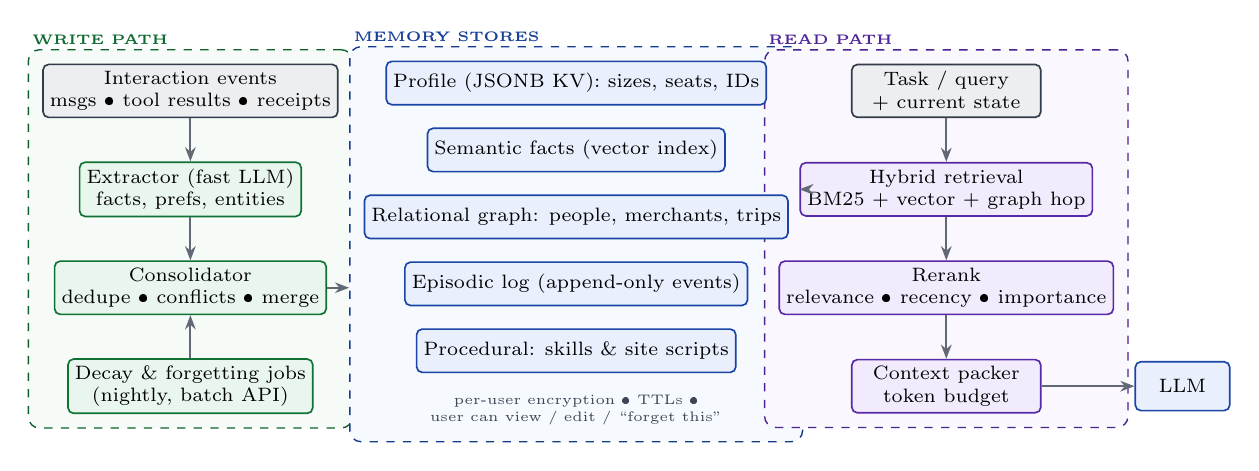
\begin{tikzpicture}
  % write path
  \node[bx=slate, minimum width=2.5cm] (ev) at (1.3,5.0) {Interaction events\\msgs \textbullet{} tool results \textbullet{} receipts};
  \node[bx=leaf, minimum width=2.5cm] (ex) at (1.3,3.75) {Extractor (fast LLM)\\facts, prefs, entities};
  \node[bx=leaf, minimum width=2.5cm] (co) at (1.3,2.5) {Consolidator\\dedupe \textbullet{} conflicts \textbullet{} merge};
  \node[bx=leaf, minimum width=2.5cm] (de) at (1.3,1.25) {Decay \& forgetting jobs\\(nightly, batch API)};
  \draw[ar] (ev) -- (ex); \draw[ar] (ex) -- (co); \draw[ar] (de) -- (co);
  \group{gw}{leaf}{(ev)(ex)(co)(de)}{WRITE PATH}
  % stores
  \foreach \n/\t/\y in {s1/{Profile (JSONB KV): sizes, seats, IDs}/5.1, s2/Semantic facts (vector index)/4.25,
      s3/{Relational graph: people, merchants, trips}/3.4, s4/Episodic log (append-only events)/2.55,
      s5/Procedural: skills \& site scripts/1.7}
    {\node[bx=accent, minimum width=3.7cm, minimum height=0.55cm] (\n) at (6.2,\y) {\t};}
  \node[nb, text width=3.8cm] (note) at (6.2,0.95) {per-user encryption \textbullet{} TTLs \textbullet{}\\user can view / edit / ``forget this''};
  \group{gs}{accent}{(s1)(s2)(s3)(s4)(s5)(note)}{MEMORY STORES}
  \draw[ar] (co.east) -- (gs.west |- co.east);
  % read path
  \node[bx=slate, minimum width=2.4cm] (q) at (10.9,5.0) {Task / query\\+ current state};
  \node[bx=violet, minimum width=2.4cm] (hr) at (10.9,3.75) {Hybrid retrieval\\BM25 + vector + graph hop};
  \node[bx=violet, minimum width=2.4cm] (rr) at (10.9,2.5) {Rerank\\relevance \textbullet{} recency \textbullet{} importance};
  \node[bx=violet, minimum width=2.4cm] (cp) at (10.9,1.25) {Context packer\\token budget};
  \draw[ar] (q) -- (hr); \draw[ar] (hr) -- (rr); \draw[ar] (rr) -- (cp);
  \group{gr}{violet}{(q)(hr)(rr)(cp)}{READ PATH}
  \draw[ar] (gs.east |- hr) -- (hr.west);
  \node[bx=accent, minimum width=1.2cm] (llm) at (13.9,1.25) {LLM};
  \draw[ar] (cp) -- (llm);
\end{tikzpicture}
\end{diagram}
\end{frame}

\begin{frame}{Memory types}
\scriptsize
\renewcommand{\arraystretch}{1.35}
\begin{tabularx}{\linewidth}{>{\bfseries\raggedright\arraybackslash}p{1.7cm} X X p{3.0cm} X}
\toprule
Type & Holds & Example & Store & Written / read\\
\midrule
Working & current task scratchpad & ``cart has 2 items, awaiting approval'' & context window + Redis & every step\\
Episodic & what happened, when & ``Sep 3: merchant agreed to extend return by 10 days'' & append-only event log (Postgres $\rightarrow$ S3) & after each step / similar tasks, audits\\
Semantic & durable facts \& preferences & ``shoe 10.5 US wide; aisle seat; vegetarian'' & pgvector + JSONB profile & post-conversation extraction / every task\\
Relational & entities and links & ``Delta SkyMiles \#; partner's birthday; merchant X policy'' & graph tables (or Neo4j later) & extraction / multi-hop questions\\
Procedural & how to get things done & ``checkout script for merchant X; negotiation playbook v3'' & versioned skill library (code + prompts) & after successful runs / planning\\
\bottomrule
\end{tabularx}
\vspace{6pt}
\begin{itemize}
  \item Memory writes are \textbf{proposals}: provenance (which message / page), confidence, and expiry are stored with every fact.
  \item Facts extracted from untrusted content (web, merchant emails) are tagged and never become instructions.
\end{itemize}
\end{frame}

% ---------------------------------------------------------------------
\begin{frame}{Tool layer: API first, browser second, human last}
\begin{columns}[c]
\column{0.55\textwidth}
\begin{diagram}
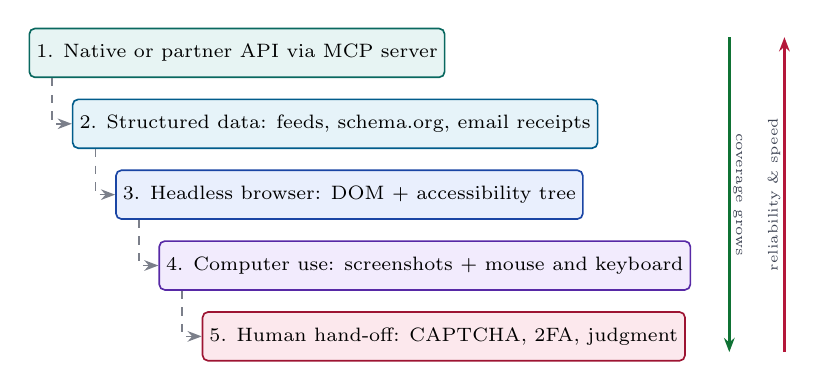
\begin{tikzpicture}
  \foreach \i/\t/\c in {0/{1. Native or partner API via MCP server}/teal, 1/{2. Structured data: feeds, schema.org, email receipts}/sky,
                        2/3. Headless browser: DOM + accessibility tree/accent, 3/{4. Computer use: screenshots + mouse and keyboard}/violet,
                        4/{5. Human hand-off: CAPTCHA, 2FA, judgment}/rose}
    {\node[bx=\c, minimum width=4.6cm, anchor=west] (s\i) at (\i*0.55, -\i*0.9) {\t};}
  \foreach \i/\j in {0/1,1/2,2/3,3/4}{\draw[dsh] (s\i.south west) ++(0.3,0) |- (s\j.west);}
  \draw[->, line width=1pt, leaf!70!black] (8.9,0.2) -- node[nb, rotate=-90, above]{coverage grows} (8.9,-3.8);
  \draw[->, line width=1pt, rose!80!black] (9.6,-3.8) -- node[nb, rotate=90, above]{reliability \& speed} (9.6,0.2);
\end{tikzpicture}
\end{diagram}
\column{0.45\textwidth}
\small
\begin{itemize}
  \item Every capability is exposed as a \textbf{typed tool} (MCP) with scopes, rate limits and idempotency.
  \item The planner picks the \textbf{highest rung} that covers the site; it falls down a rung on failure.
  \item Successful browser runs are \textbf{compiled into scripts} (procedural memory) so rung 3 behaves like rung 1 next time.
  \item Human hand-off is a first-class tool: live browser view streamed to the user's phone.
\end{itemize}
\end{columns}
\end{frame}

\begin{frame}{Tool catalog (example vendors per category)}
\scriptsize
\renewcommand{\arraystretch}{1.3}
\begin{tabularx}{\linewidth}{>{\bfseries\raggedright\arraybackslash}p{2.4cm} X}
\toprule
Category & Building blocks\\
\midrule
Search \& fetch & Claude web search / web fetch server tools; Brave, Exa or Tavily search APIs; readability extraction\\
Browser & Playwright over CDP; hosted browsers (Browserbase, Steel, Anchor) or self-hosted Chromium in Firecracker / gVisor sandboxes; computer-use tool for pixel-level control\\
Commerce & Shopify Storefront / catalog APIs, retailer \& affiliate product APIs, Agentic Commerce Protocol (ACP) merchants, browser checkout as fallback, order-tracking via email parsing\\
Travel & Duffel (flights incl. NDC content), GDS (Amadeus, Sabre), hotel APIs (Expedia Rapid, Booking.com), flight-status feeds for delays \& rebooking\\
Communication & Gmail API / Microsoft Graph (mail), Twilio (SMS + voice / SIP), realtime speech-to-speech models for phone calls, merchant live chat via browser\\
Payments & Stripe Issuing virtual cards with real-time authorization; network agent tokens (Visa Intelligent Commerce, Mastercard Agent Pay); AP2 payment mandates as they mature\\
Personal data & Google / Microsoft calendar \& contacts, Plaid (transactions for price-drop \& subscription detection), encrypted document vault (passport, receipts)\\
Protocols & MCP (agent $\leftrightarrow$ tools), A2A (agent $\leftrightarrow$ agent), ACP / AP2 (checkout \& payment authorization)\\
\bottomrule
\end{tabularx}
\end{frame}

% ---------------------------------------------------------------------
\begin{frame}{Browser agent subsystem}
\begin{diagram}
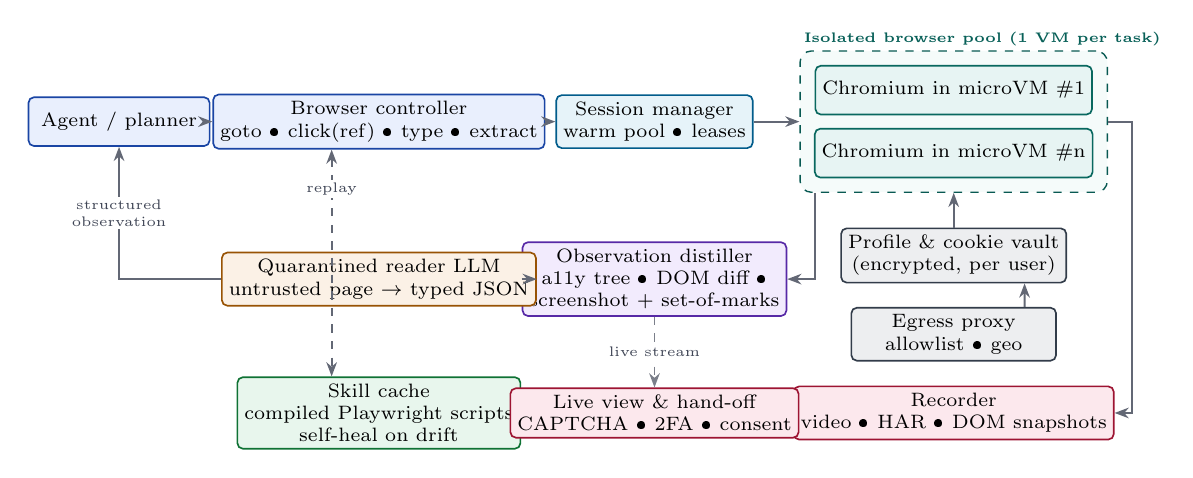
\begin{tikzpicture}
  \node[bx=accent, minimum width=2.3cm] (ag) at (1.2,4.9) {Agent / planner};
  \node[bx=accent, minimum width=2.6cm] (ctl) at (4.5,4.9) {Browser controller\\goto \textbullet{} click(ref) \textbullet{} type \textbullet{} extract};
  \node[bx=sky, minimum width=2.4cm] (sm) at (8.0,4.9) {Session manager\\warm pool \textbullet{} leases};
  \node[bx=teal, minimum width=2.6cm] (vm1) at (11.8,5.3) {Chromium in microVM \#1};
  \node[bx=teal, minimum width=2.6cm] (vm2) at (11.8,4.5) {Chromium in microVM \#n};
  \group{pool}{teal}{(vm1)(vm2)}{Isolated browser pool (1 VM per task)}
  \node[bx=slate, minimum width=2.6cm] (vault) at (11.8,3.2) {Profile \& cookie vault\\(encrypted, per user)};
  \node[bx=slate, minimum width=2.6cm] (px) at (11.8,2.2) {Egress proxy\\allowlist \textbullet{} geo};
  \node[bx=rose, minimum width=2.6cm] (rec) at (11.8,1.2) {Recorder\\video \textbullet{} HAR \textbullet{} DOM snapshots};
  \node[bx=violet, minimum width=2.6cm] (dist) at (8.0,2.9) {Observation distiller\\a11y tree \textbullet{} DOM diff \textbullet{}\\screenshot + set-of-marks};
  \node[bx=amber, minimum width=2.6cm] (qr) at (4.5,2.9) {Quarantined reader LLM\\untrusted page $\rightarrow$ typed JSON};
  \node[bx=leaf, minimum width=2.6cm] (sk) at (4.5,1.2) {Skill cache\\compiled Playwright scripts\\self-heal on drift};
  \node[bx=rose, minimum width=2.6cm] (hv) at (8.0,1.2) {Live view \& hand-off\\CAPTCHA \textbullet{} 2FA \textbullet{} consent};
  \draw[ar] (ag) -- (ctl); \draw[ar] (ctl) -- (sm); \draw[ar] (sm) -- (pool.west |- sm);
  \draw[ar] (pool.south west) ++(0.2,0) |- (dist.east);
  \draw[ar] (dist) -- (qr);
  \draw[ar] (qr.west) -| node[lb, pos=0.75]{structured\\observation} (ag.south);
  \draw[dar, dashed] (ctl.south) ++(-0.6,0) -- node[lb]{replay} ++(0,-1.0) -| ([xshift=-0.6cm]sk.north);
  \draw[ar] (vault) -- (vault |- pool.south);
  \draw[ar] (px.north) ++(0.9,0) -- ++(0,0.25) -- ([xshift=0.9cm]vault.south);
  \draw[ar] (pool.east) -- ++(0.3,0) |- (rec.east);
  \draw[dsh] (dist.south) -- node[lb]{live stream} (hv.north);
\end{tikzpicture}
\end{diagram}
\end{frame}

% ---------------------------------------------------------------------
\begin{frame}{Safety: containing prompt injection (dual-LLM + policy engine)}
\begin{diagram}
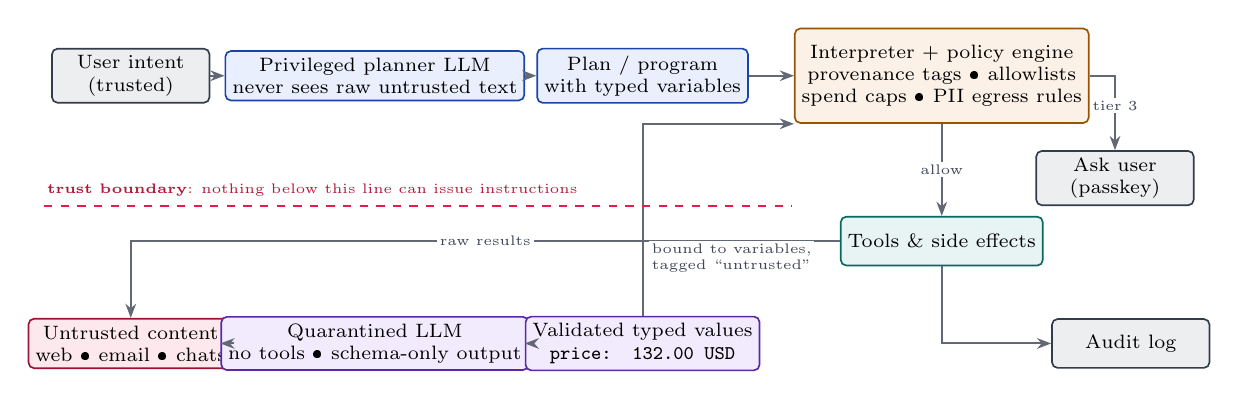
\begin{tikzpicture}
  \node[bx=slate, minimum width=2.0cm] (u) at (0.9,4.6) {User intent\\(trusted)};
  \node[bx=accent, minimum width=2.6cm] (p) at (4.0,4.6) {Privileged planner LLM\\never sees raw untrusted text};
  \node[bx=accent, minimum width=2.6cm] (prog) at (7.4,4.6) {Plan / program\\with typed variables};
  \node[bx=amber, minimum width=2.8cm, minimum height=1.2cm] (pe) at (11.2,4.6)
     {Interpreter + policy engine\\provenance tags \textbullet{} allowlists\\spend caps \textbullet{} PII egress rules};
  \node[bx=teal, minimum width=2.0cm] (tools) at (11.2,2.5) {Tools \& side effects};
  \node[bx=rose, minimum width=2.2cm] (un) at (0.9,1.2) {Untrusted content\\web \textbullet{} email \textbullet{} chats};
  \node[bx=violet, minimum width=2.6cm] (q) at (4.0,1.2) {Quarantined LLM\\no tools \textbullet{} schema-only output};
  \node[bx=violet, minimum width=2.4cm] (val) at (7.4,1.2) {Validated typed values\\\texttt{price: 132.00 USD}};
  \node[bx=slate, minimum width=2.0cm] (ask) at (13.4,3.3) {Ask user\\(passkey)};
  \node[bx=slate, minimum width=2.0cm] (log) at (13.6,1.2) {Audit log};
  \draw[ar] (u) -- (p); \draw[ar] (p) -- (prog); \draw[ar] (prog) -- (pe);
  \draw[ar] (pe) -- node[lb]{allow} (tools);
  \draw[ar] (pe.east) -| node[lb, pos=0.7]{tier 3} (ask.north);
  \draw[ar] (tools.west) -| node[lb, pos=0.25]{raw results} (un.north);
  \draw[ar] (un) -- (q); \draw[ar] (q) -- (val);
  \draw[ar] (val.north) -- node[lb, right=2pt, pos=0.3]{bound to variables,\\ tagged ``untrusted''} (val.north |- pe.south west) -- (pe.south west);
  \draw[ar] (tools) -- (tools |- log.west) -- (log.west);
  \draw[rose, dashed, line width=0.8pt] (-0.2,2.95) -- (9.3,2.95);
  \node[nb, text=rose!80!black, anchor=west] at (-0.2,3.15) {\textbf{trust boundary}: nothing below this line can issue instructions};
\end{tikzpicture}
\end{diagram}
\end{frame}

\begin{frame}{Permission tiers and injection defenses}
\begin{columns}[T]
\column{0.56\textwidth}
\scriptsize
\renewcommand{\arraystretch}{1.3}
\begin{tabularx}{\linewidth}{p{0.5cm} X p{1.7cm}}
\toprule
Tier & Actions & Policy\\
\midrule
\pill{leaf}{0} & read-only: search, browse, read email, check prices & automatic\\
\pill{sky}{1} & reversible: add to cart, draft email, hold a fare & auto + notify\\
\pill{amber}{2} & small commitments within user limits (e.g.\ $\le$\$50 at trusted merchant) & auto if policy allows\\
\pill{rose}{3} & money, irreversible, identity: checkout, ticketing, cancellations, calling on your behalf, sharing PII & explicit approval, step-up auth\\
\pill{ink}{4} & credential entry on unknown domains, deceptive claims, illegal requests & always deny\\
\bottomrule
\end{tabularx}
\column{0.44\textwidth}
\small
\textbf{Defense in depth}
\begin{itemize}
  \item Separate \textbf{instructions} (user) from \textbf{data} (world); quarantine readers.
  \item \textbf{Provenance tags} flow with every value; policy checks data flow, not just the call.
  \item Domain \& merchant \textbf{allowlists}; egress proxy blocks exfiltration.
  \item \textbf{Virtual cards} capped per task $\Rightarrow$ worst case is bounded.
  \item Injection red-team suite runs in CI on every prompt / model change.
\end{itemize}
\end{columns}
\end{frame}

% ---------------------------------------------------------------------
\begin{frame}{Money movement: per-task virtual cards}
\begin{diagram}
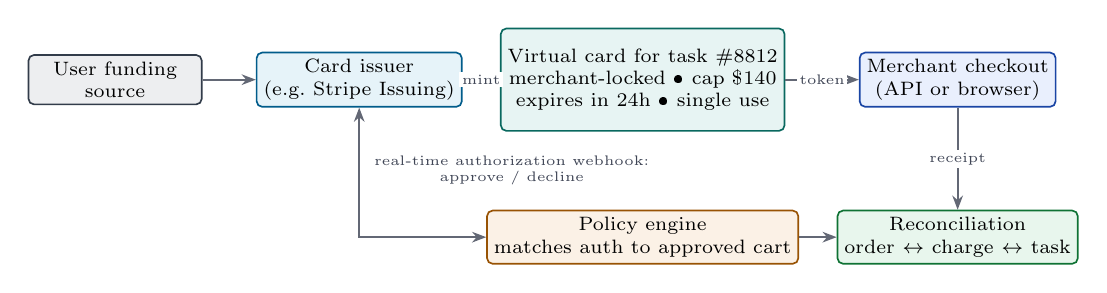
\begin{tikzpicture}
  \node[bx=slate, minimum width=2.2cm] (fund) at (0.9,3.2) {User funding\\source};
  \node[bx=sky, minimum width=2.5cm] (iss) at (4.0,3.2) {Card issuer\\(e.g.\ Stripe Issuing)};
  \node[bx=teal, minimum width=3.0cm, minimum height=1.3cm] (vc) at (7.6,3.2)
     {Virtual card for task \#8812\\merchant-locked \textbullet{} cap \$140\\expires in 24h \textbullet{} single use};
  \node[bx=accent, minimum width=2.4cm] (m) at (11.6,3.2) {Merchant checkout\\(API or browser)};
  \node[bx=amber, minimum width=3.0cm] (pe) at (7.6,1.2) {Policy engine\\matches auth to approved cart};
  \node[bx=leaf, minimum width=2.4cm] (rec) at (11.6,1.2) {Reconciliation\\order $\leftrightarrow$ charge $\leftrightarrow$ task};
  \draw[ar] (fund) -- (iss); \draw[ar] (iss) -- node[lb]{mint}(vc); \draw[ar] (vc) -- node[lb]{token}(m);
  \draw[dar] (iss.south) |- (pe.west); \node[lb, anchor=west] at (4.15,2.05) {real-time authorization webhook:\\approve / decline};
  \draw[ar] (m) -- node[lb]{receipt}(rec);
  \draw[ar] (pe) -- (rec);
\end{tikzpicture}
\end{diagram}
\small
\begin{itemize}
  \item The agent never sees the user's real card; PAN stays with the issuer $\Rightarrow$ minimal PCI scope.
  \item Authorization is checked against the \emph{approved} cart in real time -- a prompt-injected checkout for a different amount or merchant is declined.
  \item Where merchants support agentic protocols (ACP, AP2, network agent tokens) use signed mandates instead of card-not-present flows.
\end{itemize}
\end{frame}

% =====================================================================
\section{Use-case flows}
% =====================================================================
\newcommand{\lane}[3]{% x, name, colour
  \node[bx=#3, minimum width=2.1cm] at (#1,0) {#2};
  \draw[ink!25, dashed] (#1,-0.35) -- (#1,-7.7);}
\newcommand{\msg}[4]{\draw[ar] (#1,-#3) -- node[above, font=\tiny, inner sep=1pt]{#4} (#2,-#3);}
\newcommand{\self}[3]{\node[fill=white, draw=ink!30, rounded corners=1pt, font=\tiny, inner sep=1.5pt, align=center] at (#1,-#2) {#3};}

\begin{frame}{Flow 1 -- Shopping: ``Running shoes like my last pair, under \$150''}
\begin{diagram}
\begin{tikzpicture}[yscale=0.95]
  \lane{0}{User}{slate} \lane{3.3}{Agent}{accent} \lane{6.6}{Memory}{leaf} \lane{9.9}{Commerce / browser}{teal} \lane{13.2}{Payments}{sky}
  \msg{0}{3.3}{0.8}{``shoes like last pair, $<$\$150''}
  \msg{3.3}{6.6}{1.4}{size, brand, past orders?}
  \msg{6.6}{3.3}{1.95}{10.5 US wide, Brooks, returned Hoka}
  \msg{3.3}{9.9}{2.55}{search 6 merchants in parallel (API + browser)}
  \msg{9.9}{3.3}{3.1}{offers, stock, delivery, return policies}
  \self{3.3}{3.65}{rank: price, ETA, return window, merchant trust}
  \msg{3.3}{0}{4.25}{top pick \$132 + 2 alts -- approve?}
  \msg{0}{3.3}{4.8}{approve (Face ID)}
  \msg{3.3}{13.2}{5.35}{mint card: merchant-locked, \$140 cap}
  \msg{3.3}{9.9}{5.9}{checkout with token (idempotent)}
  \msg{9.9}{3.3}{6.45}{order \#, ETA}
  \msg{3.3}{6.6}{6.95}{episode + receipt + return deadline}
  \msg{3.3}{0}{7.45}{confirmed; reminder before window}
\end{tikzpicture}
\end{diagram}
\end{frame}

\begin{frame}{Flow 2 -- Travel: ``Lisbon Oct 12--19, aisle, under \$900, miles if better''}
\begin{diagram}
\begin{tikzpicture}[yscale=0.95]
  \lane{0}{User}{slate} \lane{3.3}{Agent}{accent} \lane{6.6}{Travel APIs}{teal} \lane{9.9}{Calendar / mail}{leaf} \lane{13.2}{Durable timers}{violet}
  \msg{0}{3.3}{0.8}{trip request}
  \msg{3.3}{9.9}{1.35}{conflicts? loyalty \#s from memory}
  \msg{3.3}{6.6}{1.9}{flight offers (NDC) + hotels near preferred area}
  \msg{6.6}{3.3}{2.45}{offers}
  \self{3.3}{2.95}{cash vs.\ points value, layover rules}
  \msg{3.3}{6.6}{3.5}{hold fare (where supported)}
  \msg{3.3}{0}{4.05}{itinerary \$842 + hotel -- approve?}
  \msg{0}{3.3}{4.55}{approve}
  \msg{3.3}{6.6}{5.1}{book + aisle seat $\rightarrow$ PNR / e-ticket}
  \msg{3.3}{9.9}{5.6}{add events, file confirmations}
  \msg{3.3}{13.2}{6.1}{watch: price drop, schedule change, check-in T-24h}
  \msg{13.2}{3.3}{6.65}{event: flight delayed 4h $\rightarrow$ fetch rebooking options}
  \msg{3.3}{0}{7.1}{proposal: rebook on 13:05, keep hotel}
\end{tikzpicture}
\end{diagram}
\end{frame}

\begin{frame}{Flow 3 -- Negotiating a late return (day 35 of a 30-day window)}
\begin{diagram}
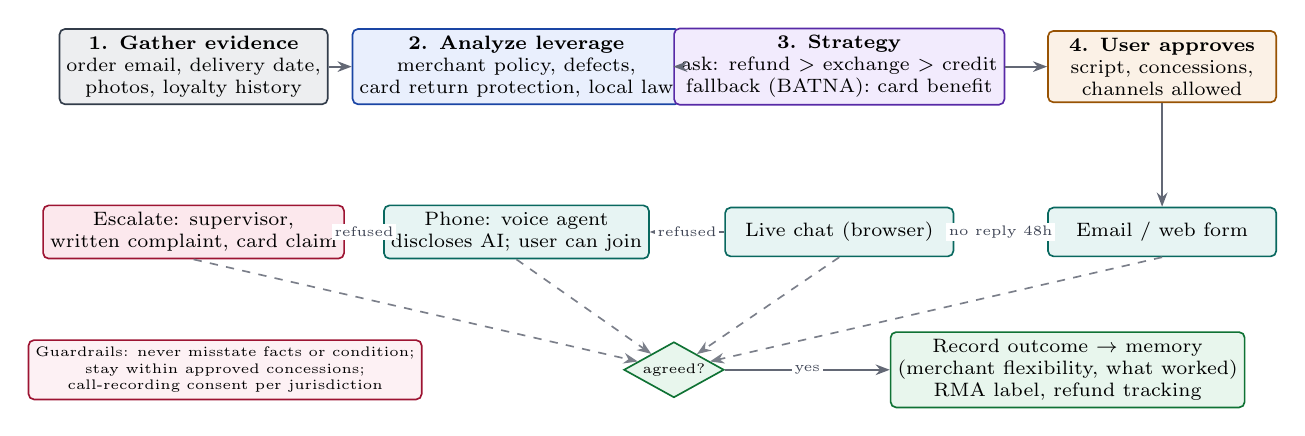
\begin{tikzpicture}
  \node[bx=slate, minimum width=2.9cm] (a) at (1.7,4.9) {\textbf{1. Gather evidence}\\order email, delivery date,\\photos, loyalty history};
  \node[bx=accent, minimum width=2.9cm] (b) at (5.8,4.9) {\textbf{2. Analyze leverage}\\merchant policy, defects,\\card return protection, local law};
  \node[bx=violet, minimum width=2.9cm] (c) at (9.9,4.9) {\textbf{3. Strategy}\\ask: refund $>$ exchange $>$ credit\\fallback (BATNA): card benefit};
  \node[bx=amber, minimum width=2.9cm] (d) at (14.0,4.9) {\textbf{4. User approves}\\script, concessions,\\channels allowed};
  \draw[ar] (a) -- (b); \draw[ar] (b) -- (c); \draw[ar] (c) -- (d);
  \node[bx=teal, minimum width=2.9cm] (e1) at (14.0,2.8) {Email / web form};
  \node[bx=teal, minimum width=2.9cm] (e2) at (9.9,2.8) {Live chat (browser)};
  \node[bx=teal, minimum width=2.9cm] (e3) at (5.8,2.8) {Phone: voice agent\\discloses AI; user can join};
  \node[bx=rose, minimum width=2.9cm] (e4) at (1.7,2.8) {Escalate: supervisor,\\written complaint, card claim};
  \draw[ar] (d) -- (e1);
  \draw[ar] (e1) -- node[lb]{no reply 48h} (e2);
  \draw[ar] (e2) -- node[lb]{refused} (e3);
  \draw[ar] (e3) -- node[lb]{refused} (e4);
  \node[dia=leaf] (ok) at (7.8,1.05) {agreed?};
  \foreach \n in {e1,e2,e3,e4}{\draw[dsh] (\n.south) -- (ok);}
  \node[bx=leaf, minimum width=3.6cm] (out) at (12.8,1.05) {Record outcome $\rightarrow$ memory\\(merchant flexibility, what worked)\\RMA label, refund tracking};
  \draw[ar] (ok) -- node[lb]{yes} (out);
  \node[bx=rose, fill=rose!6, minimum width=3.9cm, font=\tiny] (gr) at (2.1,1.05)
     {Guardrails: never misstate facts or condition;\\stay within approved concessions;\\call-recording consent per jurisdiction};
\end{tikzpicture}
\end{diagram}
\end{frame}

\begin{frame}{Negotiation playbook (what the agent actually says)}
\begin{columns}[T]
\column{0.48\textwidth}
\small
\textbf{Principles}
\begin{itemize}
  \item Lead with facts and loyalty: ``customer since 2019, 14 orders, first return request.''
  \item Cite the policy precisely, then ask for a specific, easy yes (``a one-time 10-day exception'').
  \item Offer a graceful fallback (exchange / store credit) only after the primary ask.
  \item Mention card return protection or chargeback rights only as the user-approved last step.
  \item Persistent, polite, time-boxed: durable workflow schedules follow-ups.
\end{itemize}
\column{0.52\textwidth}
\scriptsize
\begin{block}{Sample opening (email, drafted by agent, approved by user)}
Hi -- I'm an AI assistant writing on behalf of Dana Lee (order \#48213). The boots arrived Aug 18 and, unworn, are
5 days past your 30-day window because Dana was travelling. Dana has been a customer since 2019 with no prior
returns. Could you make a one-time exception and issue a return label? An exchange for size 10 would also work.
Photos of the unworn boots with tags are attached.
\end{block}
\vspace{2pt}
{\color{slate}Evaluation: success rate, concessions given, turns-to-resolution, and a ``would the user sign this?'' judge.}
\end{columns}
\end{frame}

% =====================================================================
\section{Architecture variants}
% =====================================================================
\begin{frame}{14 architecture variants at a glance}
\small
\begin{columns}[T]
\column{0.5\textwidth}
\begin{enumerate}
  \item Monolithic ReAct agent
  \item Planner -- executor -- verifier
  \item Orchestrator + specialist sub-agents
  \item Durable workflow graph (LLM at nodes)
  \item Event-driven ambient agent
  \item Computer-use / browser-native agent
  \item API-first MCP tool mesh
\end{enumerate}
\column{0.5\textwidth}
\begin{enumerate}\setcounter{enumi}{7}
  \item Local-first hybrid (on-device + cloud)
  \item Dual-LLM security architecture
  \item Agent-to-agent commerce (A2A / ACP)
  \item Voice-first agent
  \item Human-in-the-loop concierge
  \item Self-improving skill library
  \item Memory-centric ``digital twin''
\end{enumerate}
\end{columns}
\vfill
{\scriptsize\color{slate}They are not mutually exclusive: slide ``Recommended composite'' shows how to combine them.}
\end{frame}

\begin{frame}{Variants 1--2}
\variant{V1 \textbullet{} Monolithic ReAct agent}{
  \node[sbx=slate] (u) at (0.5,1.1) {User};
  \node[bx=accent, minimum width=2.2cm] (l) at (2.8,1.1) {single LLM loop\\reason $\leftrightarrow$ act};
  \draw[ar] ([xshift=0.5cm]l.north) .. controls +(0.2,0.7) and +(-0.2,0.7) .. ([xshift=-0.5cm]l.north);
  \foreach \t/\y/\k in {search/1.9/a,browser/1.1/b,checkout/0.3/c}{\node[sbx=teal, minimum width=1.3cm] (t\k) at (5.6,\y) {\t}; \draw[dar] (l.east) -- (t\k.west);}
  \draw[ar] (u) -- (l);}
{one model, one context window, all tools (tool search when there are many).}
{week-1 prototype, demos, internal tools.}
{context bloat, weak on multi-day tasks, hard to govern and evaluate.}
\hfill
\variant{V2 \textbullet{} Planner -- executor -- verifier}{
  \node[bx=accent] (p) at (0.8,1.1) {Planner\\(frontier)};
  \node[bx=teal] (e) at (3.2,1.1) {Executor\\(fast model)};
  \node[bx=amber] (v) at (5.6,1.1) {Verifier\\goal met?};
  \node[sbx=teal] (t) at (3.2,2.2) {tools};
  \draw[ar] (p) -- node[lb]{plan} (e); \draw[ar] (e) -- (v); \draw[dar] (e) -- (t);
  \draw[ar] (v.south) to[bend left=30] node[lb]{replan on failure} (p.south);}
{explicit step plan; a cheaper model executes; a verifier checks outcome before commit.}
{multi-step checkout and booking with verifiable goals.}
{replanning latency; rigid plans on dynamic sites.}
\end{frame}

\begin{frame}{Variants 3--4}
\variant{V3 \textbullet{} Orchestrator + specialist sub-agents}{
  \node[bx=accent, minimum width=2.4cm] (o) at (3.2,2.1) {Orchestrator\\intent routing, shared state};
  \foreach \t/\x/\c/\k in {Shopping/0.6/teal/a,Travel/2.35/sky/b,Negotiator/4.05/violet/c,Research/5.8/leaf/d}
    {\node[bx=\c, minimum width=1.4cm] (s\k) at (\x,0.4) {\t}; \draw[dar] (o.south) -- (s\k.north);}}
{a router delegates to domain agents with their own prompts, tools and eval suites.}
{growing teams, per-vertical ownership, parallel sub-tasks.}
{hand-off context loss; paying for several contexts per task.}
\hfill
\variant{V4 \textbullet{} Durable workflow graph}{
  \node[sbx=slate] (s) at (0.3,1.1) {start};
  \node[bx=accent] (a) at (1.6,1.1) {search\\\tiny LLM};
  \node[dia=amber] (d) at (3.2,1.1) {approve?};
  \node[bx=teal] (b) at (4.7,1.1) {book};
  \node[bx=violet] (m) at (6.1,1.1) {monitor\\\tiny timers};
  \node[bx=slate] (r) at (3.2,-0.2) {revise \tiny LLM};
  \draw[ar] (s)--(a); \draw[ar] (a)--(d); \draw[ar] (d)--node[lb]{yes}(b); \draw[ar] (b)--(m);
  \draw[ar] (d)--node[lb]{no}(r); \draw[ar] (r) -| (a);}
{deterministic state machine (Temporal / Restate) with LLM calls only at decision nodes; sagas for rollback.}
{travel, returns -- anything with money and waiting.}
{less flexible for novel, open-ended requests.}
\end{frame}

\begin{frame}{Variants 5--6}
\variant{V5 \textbullet{} Event-driven ambient agent}{
  \foreach \t/\y/\k in {inbox/1.9/a,price drop/1.1/b,flight delay/0.3/c}{\node[sbx=slate, minimum width=1.4cm] (e\k) at (0.7,\y) {\t};}
  \node[bx=sky, minimum height=1.9cm] (bus) at (2.5,1.1) {event\\bus};
  \foreach \k in {a,b,c}{\draw[ar] (e\k) -- (bus.west |- e\k);}
  \node[bx=amber] (tr) at (4.2,1.1) {triggers +\\LLM triage};
  \node[bx=accent] (ag) at (5.9,1.1) {act or\\notify};
  \draw[ar] (bus)--(tr); \draw[ar] (tr)--(ag);}
{agents wake on events (receipts, price drops, flight status, deadlines) and act or notify proactively.}
{``chief of staff'': price-adjustment refunds, check-ins, return deadlines.}
{notification fatigue; needs strict per-trigger budgets.}
\hfill
\variant{V6 \textbullet{} Computer-use / browser-native}{
  \node[bx=accent] (a) at (0.8,1.1) {agent};
  \node[bx=teal, minimum width=1.9cm] (vm) at (3.4,1.1) {Chromium\\in microVM};
  \node[bx=slate, minimum width=1.6cm] (w) at (5.8,1.1) {any website};
  \draw[ar] (a.north) to[bend left=30] node[lb]{click / type} (vm.north);
  \draw[ar] (vm.south) to[bend left=30] node[lb]{screenshot + a11y tree} (a.south);
  \draw[dar] (vm)--(w);}
{the model operates a real browser from screenshots and DOM; zero integrations required.}
{the long tail of sites with no API.}
{slowest and most expensive per task; bot defenses and ToS.}
\end{frame}

\begin{frame}{Variants 7--8}
\variant{V7 \textbullet{} API-first MCP tool mesh}{
  \node[bx=accent] (a) at (0.7,1.1) {agent};
  \node[bx=teal, minimum height=1.8cm] (h) at (2.7,1.1) {MCP\\gateway};
  \foreach \t/\y/\k in {Duffel/2.0/a,Shopify/1.55/b,Gmail/1.1/c,Calendar/0.65/d,Stripe/0.2/e}
    {\node[sbx=teal, minimum width=1.5cm] (m\k) at (5.2,\y) {\t}; \draw[ar] (h.east |- m\k) -- (m\k.west);}
  \draw[dar] (a)--(h);}
{every capability is an MCP server with typed schemas and OAuth scopes; browser only as fallback.}
{reliability, speed, auditability, low cost.}
{coverage limited to partners; integration effort per vendor.}
\hfill
\variant{V8 \textbullet{} Local-first hybrid}{
  \node[bx=leaf] (slm) at (1.0,1.6) {on-device\\small model};
  \node[bx=leaf] (pm) at (1.0,0.5) {private\\memory};
  \draw[dar] (slm)--(pm);
  \node[draw=leaf!60!black, dashed, rounded corners, fit=(slm)(pm), inner sep=3pt, label={[nb]above:phone}] (ph) {};
  \node[dia=amber] (r) at (3.3,1.1) {redact\\route};
  \node[bx=accent] (c) at (5.5,1.6) {cloud frontier\\LLM};
  \node[bx=teal] (ct) at (5.5,0.5) {cloud tools};
  \draw[ar] (ph)--(r); \draw[ar] (r)--(c); \draw[ar] (r)--(ct);}
{on-device model handles intent, PII and memory; the cloud model receives redacted context.}
{privacy-sensitive users, offline use, low latency.}
{device fragmentation, sync, weaker local reasoning.}
\end{frame}

\begin{frame}{Variants 9--10}
\variant{V9 \textbullet{} Dual-LLM security architecture}{
  \node[bx=accent] (p) at (0.8,1.8) {P-LLM\\planner};
  \node[bx=accent] (pr) at (2.6,1.8) {program};
  \node[bx=amber] (in) at (4.5,1.8) {interpreter\\+ policy};
  \node[bx=teal] (t) at (6.2,1.8) {tools};
  \node[bx=rose] (d) at (6.2,0.3) {untrusted\\data};
  \node[bx=violet] (q) at (4.5,0.3) {Q-LLM\\no tools};
  \draw[ar] (p)--(pr); \draw[ar] (pr)--(in); \draw[ar] (in)--(t); \draw[ar] (t)--(d); \draw[ar] (d)--(q);
  \draw[ar] (q)--node[lb]{typed values}(in);}
{the privileged LLM plans without ever reading untrusted text; a quarantined LLM parses pages into typed values; policy enforces data flow.}
{payments, PII, high-assurance actions.}
{engineering complexity; some tasks must reason over untrusted text.}
\hfill
\variant{V10 \textbullet{} Agent-to-agent commerce}{
  \node[bx=accent, minimum height=1.8cm] (u) at (0.9,1.1) {user's\\agent};
  \foreach \t/\y/\c/\k in {merchant agent/1.9/teal/a,airline agent/1.1/sky/b,payment network/0.3/amber/c}
    {\node[bx=\c, minimum width=2.0cm] (x\k) at (5.4,\y) {\t}; \draw[dar] (u.east |- x\k) -- (x\k.west);}
  \node[lb] at (3.15,1.1) {A2A / ACP / AP2};}
{your agent negotiates and checks out with merchant and airline agents via open protocols and signed payment mandates.}
{future-proof commerce; no scraping; structured offers.}
{early ecosystem; adversarial counter-agents.}
\end{frame}

\begin{frame}{Variants 11--12}
\variant{V11 \textbullet{} Voice-first agent}{
  \node[bx=slate] (e) at (0.8,1.7) {earbuds /\\phone};
  \node[bx=violet, minimum width=1.9cm] (rt) at (3.1,1.7) {realtime\\speech model};
  \node[bx=accent] (ac) at (5.5,1.7) {agent core\\+ tools};
  \node[bx=teal] (sip) at (3.1,0.3) {SIP / PSTN};
  \node[bx=slate] (cc) at (5.5,0.3) {merchant\\call centre};
  \draw[dar] (e)--(rt); \draw[dar] (rt)--(ac); \draw[ar] (ac.south west) -- (sip.north east); \draw[dar] (sip)--(cc);}
{realtime speech-to-speech front end; outbound calls handle customer service and reservations.}
{negotiation, reservations, hands-free use.}
{AI-call disclosure \& consent law (e.g.\ TCPA), latency, recording rules.}
\hfill
\variant{V12 \textbullet{} Human-in-the-loop concierge}{
  \node[bx=accent] (a) at (0.7,1.1) {agent};
  \node[dia=amber] (c) at (2.6,1.1) {risk /\\confidence};
  \node[bx=teal] (x) at (4.8,1.9) {execute};
  \node[bx=rose] (h) at (4.8,0.3) {operator\\queue};
  \node[bx=leaf] (tr) at (6.3,0.3) {training\\data};
  \draw[ar] (a)--(c); \draw[ar] (c)--node[lb]{high}(x); \draw[ar] (c)--node[lb]{low}(h);
  \draw[ar] (h)--(x); \draw[dsh] (h)--(tr);}
{a risk/confidence router sends hard cases to human operators who act through the same tools.}
{launch quality at small scale; building trust; labeled data.}
{operations cost; the human share must shrink over time.}
\end{frame}

\begin{frame}{Variants 13--14}
\variant{V13 \textbullet{} Self-improving skill library}{
  \node[bx=slate] (t) at (0.7,1.1) {successful\\trajectories};
  \node[bx=violet] (c) at (2.55,1.1) {skill\\compiler};
  \node[bx=leaf] (l) at (4.4,1.1) {versioned\\skill library};
  \node[bx=teal] (r) at (6.2,1.1) {replay\\(no LLM)};
  \draw[ar] (t)--(c); \draw[ar] (c)--(l); \draw[ar] (l)--(r);
  \draw[ar] (r.south) to[bend left=25] node[lb]{drift / failure $\rightarrow$ LLM repairs} (c.south);}
{trajectories become parameterized scripts, replayed deterministically; the LLM is used only when a site changes.}
{high-frequency flows at scale -- 5--20$\times$ cheaper and faster.}
{site drift; skill verification and versioning.}
\hfill
\variant{V14 \textbullet{} Memory-centric ``digital twin''}{
  \node[bx=leaf, minimum width=2.4cm, minimum height=1.1cm] (tw) at (3.2,1.1) {user model\\prefs \textbullet{} relations\\values \textbullet{} constraints};
  \node[sbx=slate, minimum width=1.4cm] (a1) at (0.7,1.9) {mail / receipts};
  \node[sbx=slate, minimum width=1.4cm] (a2) at (0.7,0.3) {calendar / bank};
  \node[sbx=amber, minimum width=1.4cm] (f) at (5.7,1.9) {user feedback};
  \node[sbx=accent, minimum width=1.4cm] (g) at (5.7,0.3) {all agents query};
  \draw[ar] (a1)--(tw); \draw[ar] (a2)--(tw); \draw[ar] (f)--(tw); \draw[ar] (tw)--(g);}
{a rich, user-editable model of preferences and constraints that every agent consults.}
{deep personalization -- the long-term moat.}
{privacy, staleness, conflicting preferences.}
\end{frame}

\begin{frame}{Comparison matrix}
\centering
\scriptsize
\renewcommand{\arraystretch}{1.12}
\begin{tabular}{l c c c c c c}
\toprule
Variant & Ease of build & Reliability & Cost efficiency & Speed & Safety / privacy & Coverage\\
\midrule
V1 Monolithic ReAct        & \rate{3} & \rate{1} & \rate{2} & \rate{2} & \rate{1} & \rate{2}\\
V2 Planner--executor--verifier & \rate{2} & \rate{2} & \rate{2} & \rate{1} & \rate{2} & \rate{2}\\
V3 Orchestrator + specialists & \rate{2} & \rate{2} & \rate{2} & \rate{2} & \rate{2} & \rate{3}\\
V4 Durable workflow graph  & \rate{2} & \rate{3} & \rate{3} & \rate{2} & \rate{3} & \rate{1}\\
V5 Event-driven ambient    & \rate{2} & \rate{2} & \rate{2} & \rate{3} & \rate{2} & \rate{2}\\
V6 Computer-use browser    & \rate{3} & \rate{1} & \rate{1} & \rate{1} & \rate{1} & \rate{3}\\
V7 API-first MCP mesh      & \rate{2} & \rate{3} & \rate{3} & \rate{3} & \rate{3} & \rate{1}\\
V8 Local-first hybrid      & \rate{1} & \rate{2} & \rate{3} & \rate{3} & \rate{3} & \rate{1}\\
V9 Dual-LLM security       & \rate{1} & \rate{3} & \rate{2} & \rate{2} & \rate{3} & \rate{2}\\
V10 Agent-to-agent         & \rate{1} & \rate{2} & \rate{3} & \rate{3} & \rate{2} & \rate{1}\\
V11 Voice-first            & \rate{1} & \rate{2} & \rate{2} & \rate{3} & \rate{2} & \rate{2}\\
V12 Human-in-the-loop      & \rate{3} & \rate{3} & \rate{1} & \rate{1} & \rate{3} & \rate{3}\\
V13 Skill library          & \rate{2} & \rate{3} & \rate{3} & \rate{3} & \rate{2} & \rate{2}\\
V14 Digital twin           & \rate{1} & \rate{2} & \rate{2} & \rate{2} & \rate{2} & \rate{2}\\
\bottomrule
\end{tabular}\\[3pt]
{\tiny\color{slate}More filled dots = better. Qualitative, relative judgments for a consumer personal-agent product.}
\end{frame}

\begin{frame}{Recommended composite}
\begin{diagram}
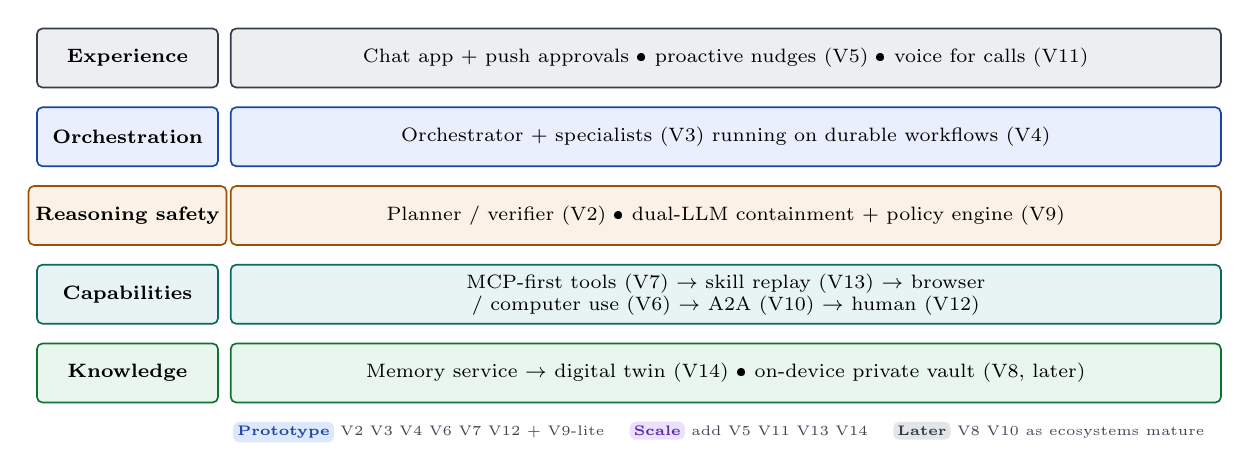
\begin{tikzpicture}
  \def\W{12.2}
  \foreach \y/\lay/\c/\txt in {
      5.0/Experience/slate/{Chat app + push approvals \textbullet{} proactive nudges (V5) \textbullet{} voice for calls (V11)},
      4.0/Orchestration/accent/{Orchestrator + specialists (V3) running on durable workflows (V4)},
      3.0/Reasoning safety/amber/{Planner / verifier (V2) \textbullet{} dual-LLM containment + policy engine (V9)},
      2.0/Capabilities/teal/{MCP-first tools (V7) $\rightarrow$ skill replay (V13) $\rightarrow$ browser / computer use (V6) $\rightarrow$ A2A (V10) $\rightarrow$ human (V12)},
      1.0/Knowledge/leaf/{Memory service $\rightarrow$ digital twin (V14) \textbullet{} on-device private vault (V8, later)}}
  {
    \node[bx=\c, minimum width=2.3cm, minimum height=0.75cm, font=\scriptsize\bfseries] at (0,\y) {\lay};
    \node[bx=\c, text width=12.4cm, minimum height=0.75cm, anchor=west] at (1.3,\y) {\txt};
  }
  \node[nb, anchor=west] at (1.3,0.25) {\pill{accent}{Prototype} V2 V3 V4 V6 V7 V12 + V9-lite
      \quad \pill{violet}{Scale} add V5 V11 V13 V14 \quad \pill{slate}{Later} V8 V10 as ecosystems mature};
\end{tikzpicture}
\end{diagram}
\end{frame}

% =====================================================================
\section{Prototype stack}
% =====================================================================
\begin{frame}{Prototype goals (0 $\rightarrow$ thousands of users)}
\begin{columns}[T]
\column{0.5\textwidth}
\small
\textbf{Scope}
\begin{itemize}
  \item 1,000--5,000 invited users, US only, one cloud region.
  \item Three verticals: shopping, travel, returns \& customer service.
  \item Mobile app + web; approvals via push notification + Face ID / passkey.
  \item Human-in-the-loop operators review risky or low-confidence steps.
\end{itemize}
\column{0.5\textwidth}
\small
\textbf{Targets}
\begin{itemize}
  \item Task success $\ge$ 80\% (with HITL), $\ge$ 65\% fully autonomous.
  \item Zero unauthorized spend (hard caps via virtual cards).
  \item First response $<$ 2\,s; simple tasks done $<$ 3\,min.
  \item 4--6 engineers, 12 weeks, mostly managed services.
  \item Every task fully traced and replayable.
\end{itemize}
\end{columns}
\end{frame}

\begin{frame}{Prototype architecture (single region, managed services)}
\begin{diagram}
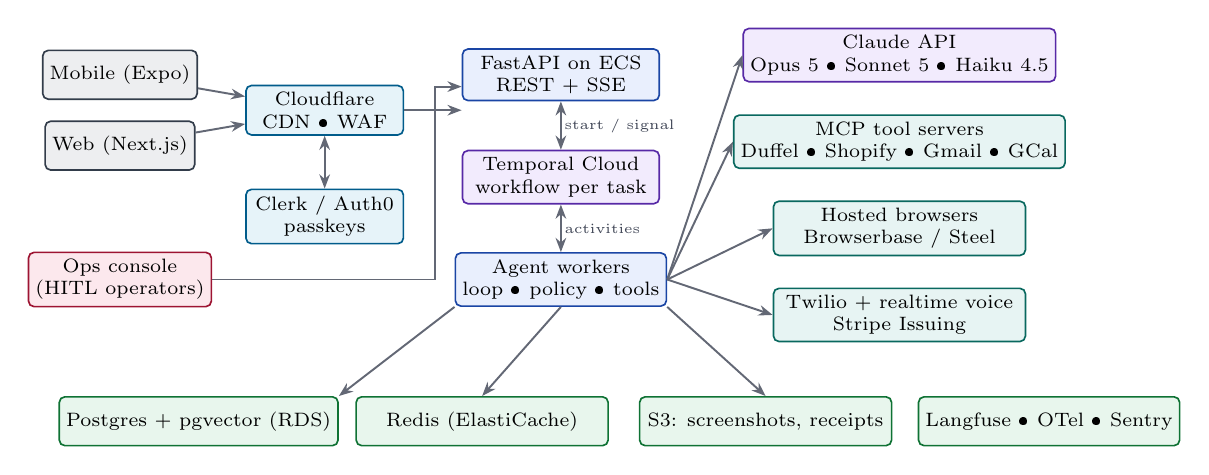
\begin{tikzpicture}
  \node[bx=slate, minimum width=1.9cm] (mob) at (1.0,4.9) {Mobile (Expo)};
  \node[bx=slate, minimum width=1.9cm] (web) at (1.0,4.0) {Web (Next.js)};
  \node[bx=rose, minimum width=1.9cm] (ops) at (1.0,2.3) {Ops console\\(HITL operators)};
  \node[bx=sky, minimum width=2.0cm] (edge) at (3.6,4.45) {Cloudflare\\CDN \textbullet{} WAF};
  \node[bx=sky, minimum width=2.0cm] (auth) at (3.6,3.1) {Clerk / Auth0\\passkeys};
  \node[bx=accent, minimum width=2.5cm] (api) at (6.6,4.9) {FastAPI on ECS\\REST + SSE};
  \node[bx=violet, minimum width=2.5cm] (tmp) at (6.6,3.6) {Temporal Cloud\\workflow per task};
  \node[bx=accent, minimum width=2.5cm] (wk) at (6.6,2.3) {Agent workers\\loop \textbullet{} policy \textbullet{} tools};
  \node[bx=violet, minimum width=3.2cm] (llm) at (10.9,5.15) {Claude API\\Opus 5 \textbullet{} Sonnet 5 \textbullet{} Haiku 4.5};
  \node[bx=teal, minimum width=3.2cm] (mcp) at (10.9,4.05) {MCP tool servers\\Duffel \textbullet{} Shopify \textbullet{} Gmail \textbullet{} GCal};
  \node[bx=teal, minimum width=3.2cm] (br) at (10.9,2.95) {Hosted browsers\\Browserbase / Steel};
  \node[bx=teal, minimum width=3.2cm] (vo) at (10.9,1.85) {Twilio + realtime voice\\Stripe Issuing};
  \foreach \n/\t/\x in {pg/Postgres + pgvector (RDS)/2.0, rd/Redis (ElastiCache)/5.6, s3/{S3: screenshots, receipts}/9.2, obs/Langfuse \textbullet{} OTel \textbullet{} Sentry/12.8}
    {\node[bx=leaf, minimum width=3.2cm] (\n) at (\x,0.5) {\t};}
  \draw[ar] (mob) -- (edge); \draw[ar] (web) -- (edge); \draw[ar] (edge) -- (api.west |- edge);
  \draw[dar] (edge) -- (auth);
  \draw[dar] (api) -- node[lb, right]{start / signal}(tmp); \draw[dar] (tmp) -- node[lb, right]{activities}(wk);
  \foreach \n in {llm,mcp,br,vo}{\draw[ar] (wk.east) -- (\n.west);}
  \draw[ar] (ops.east) -- (5.0,2.3) |- ([yshift=-0.15cm]api.west);
  \draw[ar] (wk.south) -- (rd.north);
  \draw[ar] (wk.south west) -- (pg.north east);
  \draw[ar] (wk.south east) -- (s3.north);
\end{tikzpicture}
\end{diagram}
\end{frame}

\begin{frame}{Prototype stack in detail (1/2)}
\scriptsize
\renewcommand{\arraystretch}{1.3}
\begin{tabularx}{\linewidth}{>{\bfseries\raggedright\arraybackslash}p{2.0cm} X p{2.9cm} p{2.2cm}}
\toprule
Layer & Choice & Why & Alternatives\\
\midrule
Clients & Expo / React Native app + Next.js web; SSE streaming; Expo push notifications; biometric approval via passkeys & one TypeScript codebase; approvals where the user is & Swift / Kotlin native\\
API & Python 3.12, FastAPI + Pydantic v2, uvicorn; REST + SSE; OpenAPI-generated TS client & richest LLM / agent ecosystem & TypeScript (Hono)\\
Agent runtime & own loop on the Anthropic SDK (tool runner hooks for approval gates); runs inside Temporal activities; MCP clients for tools & full control over policy, caching, retries & LangGraph, Pydantic AI\\
Models & Claude Opus 5 for planning \& negotiation; Sonnet 5 for most tool steps and browser control; Haiku 4.5 for extraction, classification, memory; prompt caching on; Batch API for nightly memory jobs & quality where it matters, cost everywhere else & multi-provider router later\\
Durable execution & Temporal Cloud: one workflow per task; signals for approvals; timers for follow-ups; activities for tool calls with retries & days-long tasks survive deploys \& crashes & Restate, Inngest, DBOS\\
Streaming \& jobs & Redis pub/sub to stream steps to the UI; Temporal schedules for price-watch \& reminders & simple, few moving parts & NATS\\
\bottomrule
\end{tabularx}
\end{frame}

\begin{frame}{Prototype stack in detail (2/2)}
\scriptsize
\renewcommand{\arraystretch}{1.08}
\begin{tabularx}{\linewidth}{>{\bfseries\raggedright\arraybackslash}p{2.0cm} X p{2.9cm} p{2.2cm}}
\toprule
Layer & Choice & Why & Alternatives\\
\midrule
Memory & Postgres 16 + pgvector (HNSW), JSONB profile, entity / edge tables, row-level security by user; Redis for working memory; S3 for artifacts & one database to operate & Turbopuffer, Neo4j (later)\\
Browser & Playwright over CDP to hosted browsers with session recording and live view for hand-off; a11y-tree + screenshot observations & no fleet to operate yet & self-hosted Chromium\\
Integrations & one MCP server per integration (Python FastMCP): Duffel, Shopify, Gmail / Graph, Google Calendar, Twilio, Stripe Issuing & typed, scoped, reusable & direct SDK calls\\
Payments & Stripe Issuing virtual cards + real-time authorization webhook into the policy engine; Stripe Billing for subscriptions & bounded worst case; tiny PCI scope & Lithic, Marqeta\\
Identity \& secrets & Clerk / Auth0 with passkeys; OAuth refresh tokens encrypted with per-user data keys (AWS KMS envelope encryption); step-up auth for tier-3 actions & least privilege & WorkOS, Vault\\
Observability \& evals & OpenTelemetry $\rightarrow$ Grafana; Langfuse for LLM traces \& cost; Sentry; pytest eval suites with LLM judges; browser video replays & debug any task end-to-end & LangSmith, Braintrust\\
Infra \& delivery & AWS: ECS Fargate, RDS, ElastiCache, S3; Terraform; GitHub Actions; GrowthBook feature flags; prompt \& model versions in git & boring and fast & Fly.io, GCP\\
\bottomrule
\end{tabularx}
\end{frame}

\begin{frame}[fragile]{Code sketch: one task = one durable workflow}
\begin{columns}[T]
\column{0.62\textwidth}
\begin{lstlisting}[basicstyle=\ttfamily\fontsize{5.4}{6.2}\selectfont]
@workflow.defn
class PersonalTask:
    def __init__(self): self.approvals: dict[str, bool] = {}
    @workflow.run
    async def run(self, task: TaskSpec) -> Outcome:
        ctx = await act(build_context, task)   # profile+memories+tools
        while not ctx.done:
            step = await act(llm_step, ctx)    # Claude: next tool calls
            for call in step.tool_calls:
                verdict = await act(policy_check, call, ctx)
                if verdict.deny:
                    ctx.add_denial(call); continue
                if verdict.needs_approval:     # push + passkey
                    await act(request_approval, call)
                    await workflow.wait_condition(
                        lambda: call.id in self.approvals,
                        timeout=timedelta(days=2))
                    if not self.approvals[call.id]:
                        ctx.add_denial(call); continue
                result = await act(run_tool, call,
                                   idem_key=f"{task.id}:{call.id}")
                ctx.observe(result)
            if ctx.waiting_on_merchant:        # e.g. return email
                await workflow.sleep(timedelta(hours=48))
        await act(write_memories, ctx)
        return ctx.outcome
    @workflow.signal
    def approve(self, call_id: str, ok: bool):
        self.approvals[call_id] = ok
\end{lstlisting}
\column{0.36\textwidth}
\small
\begin{itemize}
  \item \texttt{act} = Temporal activity with retries \& timeouts; LLM and tool calls are activities, so a crash replays from history, not from scratch.
  \item Approvals are \textbf{signals}; waiting two days costs nothing.
  \item \textbf{Idempotency key} per tool call prevents double purchases on retry.
  \item The loop is the same for every vertical; specialists differ in prompts, tools and policies.
\end{itemize}
\end{columns}
\end{frame}

\begin{frame}{12-week build plan}
\begin{diagram}
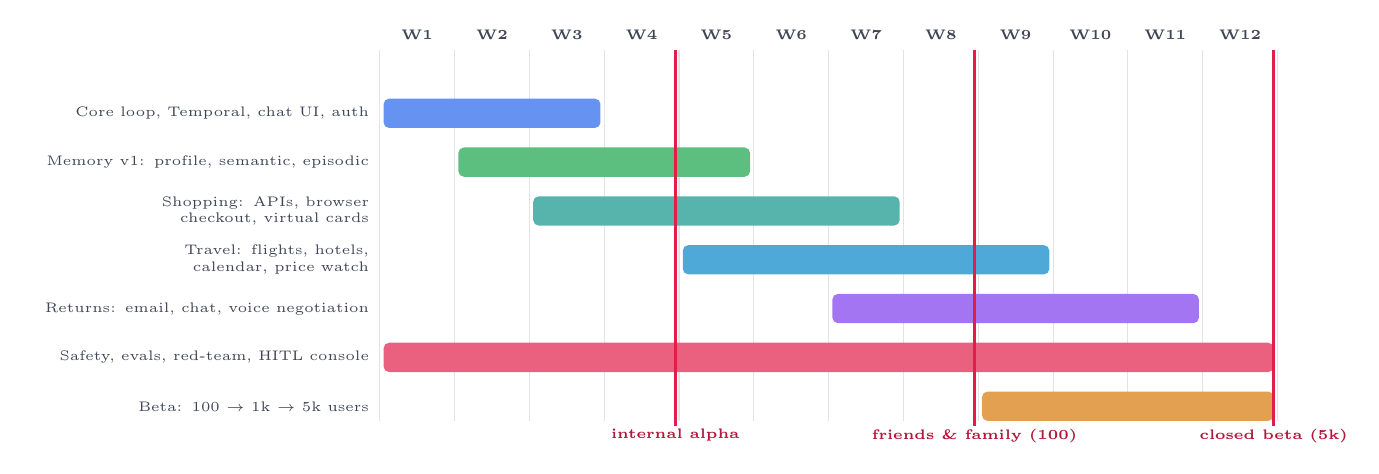
\begin{tikzpicture}[x=0.95cm, y=0.62cm]
  \foreach \w in {1,...,12}{\node[nb, font=\tiny\bfseries] at (\w+2.5,0.6) {W\w}; \draw[ink!12] (\w+2,0.3) -- (\w+2,-7.3);}
  \draw[ink!12] (15,0.3) -- (15,-7.3);
  \foreach \r/\t/\s/\e/\c in {
      1/{Core loop, Temporal, chat UI, auth}/1/3/accent,
      2/{Memory v1: profile, semantic, episodic}/2/5/leaf,
      3/{Shopping: APIs, browser checkout, virtual cards}/3/7/teal,
      4/{Travel: flights, hotels, calendar, price watch}/5/9/sky,
      5/{Returns: email, chat, voice negotiation}/7/11/violet,
      6/{Safety, evals, red-team, HITL console}/1/12/rose,
      7/Beta: 100 $\rightarrow$ 1k $\rightarrow$ 5k users/9/12/amber}
  {
    \node[nb, anchor=east, text width=4.3cm, align=right] at (2.9,-\r) {\t};
    \fill[\c!70, rounded corners=2pt] (\s+2.05,-\r-0.3) rectangle (\e+2.95,-\r+0.3);
  }
  \foreach \w/\t in {4/internal alpha, 8/friends \& family (100), 12/closed beta (5k)}
    {\draw[rose, line width=1pt] (\w+2.95,0.3) -- (\w+2.95,-7.4); \node[nb, text=rose!80!black, font=\tiny\bfseries, anchor=north] at (\w+2.95,-7.4) {\t};}
\end{tikzpicture}
\end{diagram}
\end{frame}

\begin{frame}{Prototype capacity and cost (order of magnitude)}
\begin{columns}[T]
\column{0.5\textwidth}
\small
\textbf{Load assumptions (5,000 users)}
\begin{itemize}
  \item 40\% weekly active $\times$ 10 tasks / week $\approx$ 3k tasks / day ($<$1 task/s).
  \item Per task: $\sim$12 LLM calls, $\sim$25k input tokens each ($\sim$80\% cache reads), $\sim$800 output tokens.
  \item 30\% of tasks use a browser for $\sim$4 min; 1\% place a phone call.
\end{itemize}
\textbf{LLM cost per task}
\begin{itemize}
  \item Sonnet 5 at \$2 / \$10 per M tokens (in / out), cache reads $\sim$0.1$\times$: $\approx$ \$0.02 per call $\rightarrow$ \$0.25.
  \item 2 Opus 5 planning / negotiation calls: $\approx$ \$0.15--0.20.
  \item $\Rightarrow$ roughly \textbf{\$0.40--0.50 per task} before optimization.
\end{itemize}
\column{0.5\textwidth}
\small
\textbf{Monthly run-rate}\\[3pt]
\scriptsize
\begin{tabular}{l r}
\toprule
Item & \$ / month\\
\midrule
LLM tokens ($\sim$90k tasks) & 35k--45k\\
Hosted browsers & 1k--3k\\
Voice \& telephony & 1k--2k\\
Temporal Cloud & 1k--2k\\
AWS (ECS, RDS, Redis, S3) & 3k--6k\\
Observability, auth, misc SaaS & 1k--3k\\
HITL operators (2--4 FTE) & 25k--50k\\
\midrule
\textbf{Total} & \textbf{$\sim$70k--110k}\\
\bottomrule
\end{tabular}\\[4pt]
{\small $\approx$ \$15--20 per active user / month $\Rightarrow$ price at \$20--30 / month with usage caps, and start cost-down work before scaling.}
\end{columns}
\end{frame}

% =====================================================================
\section{Scaling to millions}
% =====================================================================
\begin{frame}{Scaling phases: what changes at each order of magnitude}
\begin{diagram}
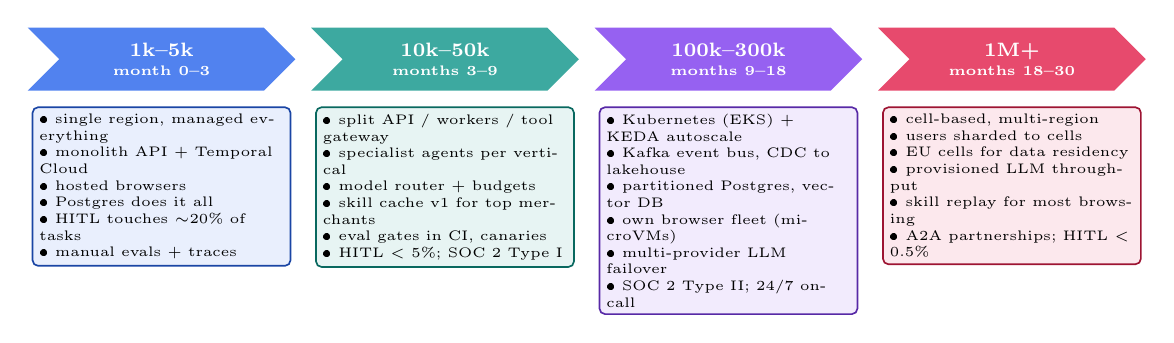
\begin{tikzpicture}
  \foreach \i/\t/\s/\c in {0/1k--5k/month 0--3/accent, 1/10k--50k/months 3--9/teal, 2/100k--300k/months 9--18/violet, 3/1M+/months 18--30/rose}
    {\node[signal, signal to=east, signal from=west, fill=\c!80, text=white, font=\scriptsize\bfseries,
           minimum width=3.4cm, minimum height=0.8cm, align=center] (h\i) at (\i*3.6,5) {\t\\[-1pt]{\tiny\s}};}
  \node[bx=accent, text width=3.1cm, align=left, font=\tiny, anchor=north] at (0,4.4) {
    \textbullet{} single region, managed everything\\
    \textbullet{} monolith API + Temporal Cloud\\
    \textbullet{} hosted browsers\\
    \textbullet{} Postgres does it all\\
    \textbullet{} HITL touches $\sim$20\% of tasks\\
    \textbullet{} manual evals + traces};
  \node[bx=teal, text width=3.1cm, align=left, font=\tiny, anchor=north] at (3.6,4.4) {
    \textbullet{} split API / workers / tool gateway\\
    \textbullet{} specialist agents per vertical\\
    \textbullet{} model router + budgets\\
    \textbullet{} skill cache v1 for top merchants\\
    \textbullet{} eval gates in CI, canaries\\
    \textbullet{} HITL $<$ 5\%; SOC 2 Type I};
  \node[bx=violet, text width=3.1cm, align=left, font=\tiny, anchor=north] at (7.2,4.4) {
    \textbullet{} Kubernetes (EKS) + KEDA autoscale\\
    \textbullet{} Kafka event bus, CDC to lakehouse\\
    \textbullet{} partitioned Postgres, vector DB\\
    \textbullet{} own browser fleet (microVMs)\\
    \textbullet{} multi-provider LLM failover\\
    \textbullet{} SOC 2 Type II; 24/7 on-call};
  \node[bx=rose, text width=3.1cm, align=left, font=\tiny, anchor=north] at (10.8,4.4) {
    \textbullet{} cell-based, multi-region\\
    \textbullet{} users sharded to cells\\
    \textbullet{} EU cells for data residency\\
    \textbullet{} provisioned LLM throughput\\
    \textbullet{} skill replay for most browsing\\
    \textbullet{} A2A partnerships; HITL $<$ 0.5\%};
\end{tikzpicture}
\end{diagram}
\end{frame}

\begin{frame}{Capacity math for 1 million users}
\begin{columns}[T]
\column{0.52\textwidth}
\small
\textbf{Traffic}
\begin{itemize}
  \item 1M MAU, 35\% daily active, 3 tasks / DAU / day $\Rightarrow$ $\sim$1M tasks / day.
  \item $\approx$ 12 tasks/s average, $\sim$60/s at peak (5$\times$).
\end{itemize}
\textbf{LLM}
\begin{itemize}
  \item 12 calls / task $\Rightarrow$ $\sim$150 calls/s average, $\sim$700/s peak.
  \item $\sim$300B input tokens / day (must be $\ge$90\% cache reads) and $\sim$10B output tokens / day.
  \item Needs negotiated / provisioned throughput and multi-provider capacity.
\end{itemize}
\column{0.48\textwidth}
\small
\textbf{Browsers \& voice}
\begin{itemize}
  \item 30\% of tasks $\times$ 4 min $\Rightarrow$ $\sim$850 concurrent sessions average, $\sim$4k peak (skill replay cuts this 5--10$\times$).
  \item 1\% of tasks $\times$ 8 min calls $\Rightarrow$ $\sim$80k call-minutes / day.
\end{itemize}
\textbf{State}
\begin{itemize}
  \item $\sim$1M workflows started / day; 5--10M long-lived (price watches, return follow-ups).
  \item Memory: thousands of items / user / year $\Rightarrow$ billions of vectors -- always queried per user.
\end{itemize}
\end{columns}
\end{frame}

\begin{frame}{Million-user architecture: cells, regions, shared platform}
\begin{diagram}
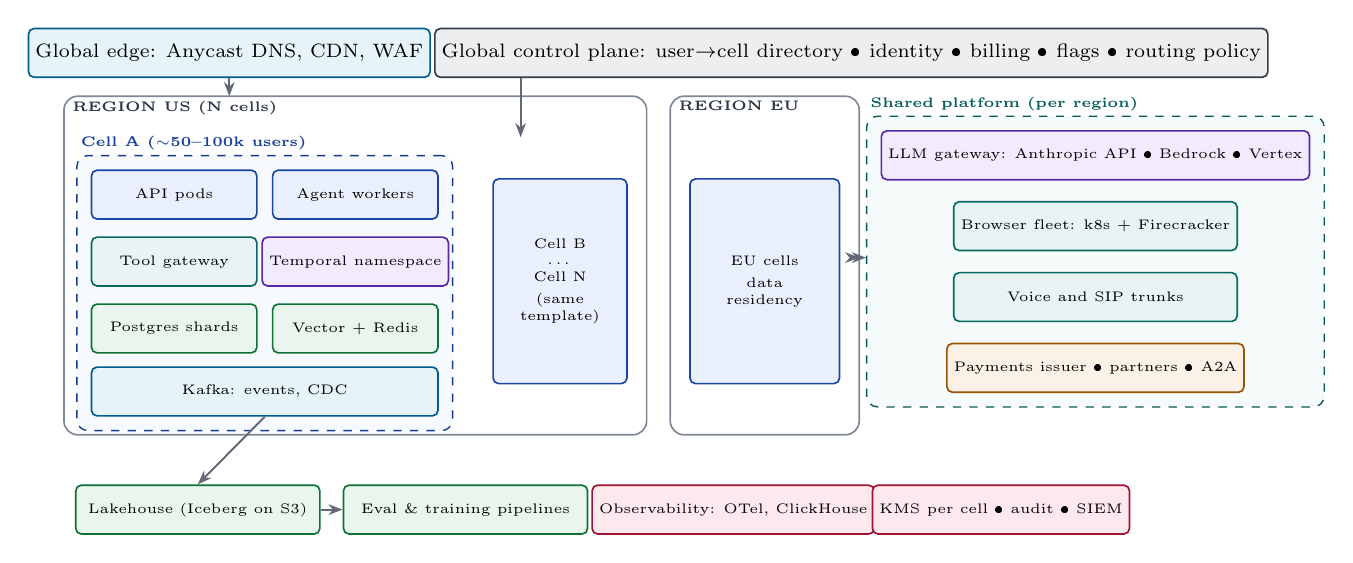
\begin{tikzpicture}
  % global
  \node[bx=sky, minimum width=4.2cm] (edge) at (2.0,6.6) {Global edge: Anycast DNS, CDN, WAF};
  \node[bx=slate, minimum width=8.4cm] (cp) at (9.9,6.6) {Global control plane: user$\rightarrow$cell directory \textbullet{} identity \textbullet{} billing \textbullet{} flags \textbullet{} routing policy};
  % region US
  \draw[slate!70, rounded corners=5pt, line width=0.6pt] (-0.1,1.75) rectangle (7.3,6.05);
  \node[gl=slate, anchor=north west] at (-0.05,6.05) {REGION US (N cells)};
  \foreach \n/\t/\x/\y/\c in {api/API pods/1.3/4.8/accent, wk/Agent workers/3.6/4.8/accent, tg/Tool gateway/1.3/3.95/teal,
       tp/Temporal namespace/3.6/3.95/violet, pg/Postgres shards/1.3/3.1/leaf, vr/Vector + Redis/3.6/3.1/leaf}
    {\node[bx=\c, minimum width=2.1cm, font=\tiny] (\n) at (\x,\y) {\t};}
  \node[bx=sky, minimum width=4.4cm, font=\tiny] (kf) at (2.45,2.3) {Kafka: events, CDC};
  \group{cella}{accent}{(api)(vr)(kf)}{Cell A ($\sim$50--100k users)}
  \node[bx=accent, minimum width=1.7cm, minimum height=2.6cm, font=\tiny] (cellb) at (6.2,3.7) {Cell B\\\ldots\\Cell N\\[2pt](same\\template)};
  % region EU
  \draw[slate!70, rounded corners=5pt, line width=0.6pt] (7.6,1.75) rectangle (10.0,6.05);
  \node[gl=slate, anchor=north west] at (7.65,6.05) {REGION EU};
  \node[bx=accent, minimum width=1.9cm, minimum height=2.6cm, font=\tiny] (eu) at (8.8,3.7) {EU cells\\[2pt]data\\residency};
  % shared
  \foreach \n/\t/\y/\c in {llm/LLM gateway: Anthropic API \textbullet{} Bedrock \textbullet{} Vertex/5.3/violet,
                           bf/Browser fleet: k8s + Firecracker/4.4/teal,
                           vc/{Voice and SIP trunks}/3.5/teal,
                           pay/Payments issuer \textbullet{} partners \textbullet{} A2A/2.6/amber}
    {\node[bx=\c, minimum width=3.6cm, font=\tiny] (\n) at (13.0,\y) {\t};}
  \group{sh}{teal}{(llm)(pay)}{Shared platform (per region)}
  % data platform
  \node[bx=leaf, minimum width=3.1cm, font=\tiny] (lake) at (1.6,0.8) {Lakehouse (Iceberg on S3)};
  \node[bx=leaf, minimum width=3.1cm, font=\tiny] (ev) at (5.0,0.8) {Eval \& training pipelines};
  \node[bx=rose, minimum width=3.1cm, font=\tiny] (ob) at (8.4,0.8) {Observability: OTel, ClickHouse};
  \node[bx=rose, minimum width=3.1cm, font=\tiny] (sec) at (11.8,0.8) {KMS per cell \textbullet{} audit \textbullet{} SIEM};
  \draw[ar] (edge) -- (edge |- 0,6.05);
  \draw[ar] (cp.south) ++(-4.2,0) -- ++(0,-0.75);
  \draw[dar] (10.0,4.0) -- (sh.west |- 0,4.0);
  \draw[ar] (kf.south) -- (lake.north);
  \draw[ar] (lake) -- (ev);
\end{tikzpicture}
\end{diagram}
\end{frame}

\begin{frame}{Cell design principles}
\begin{columns}[T]
\column{0.5\textwidth}
\small
\begin{itemize}
  \item A \textbf{cell} is a complete, independent copy of the stack serving a fixed set of users (50--100k). Blast radius of any failure = one cell.
  \item Users are \textbf{pinned to cells} via the global directory; moving a user = replay their data into another cell.
  \item Cells scale out, not up: new cohort $\Rightarrow$ new cell from the same Terraform / Helm template.
  \item Rollouts go cell by cell (canary cell first) for code, prompts and model versions.
\end{itemize}
\column{0.5\textwidth}
\small
\begin{itemize}
  \item \textbf{Shared, stateless services} stay regional: LLM gateway, browser fleet, telephony, payments.
  \item \textbf{Temporal}: one namespace per cell; workers autoscaled by KEDA on task-queue backlog.
  \item \textbf{Postgres}: Aurora or Citus, sharded by \texttt{user\_id}; episodic logs older than 90 days tier to Iceberg.
  \item \textbf{Vector}: per-user namespaces in a multi-tenant vector store (Turbopuffer / Pinecone serverless) or partitioned pgvector -- every query is user-scoped, so indexes stay tiny.
\end{itemize}
\end{columns}
\end{frame}

\begin{frame}{LLM cost-down at scale: \$0.45 $\rightarrow$ $\sim$\$0.09 per task}
\begin{columns}[c]
\column{0.55\textwidth}
\begin{diagram}
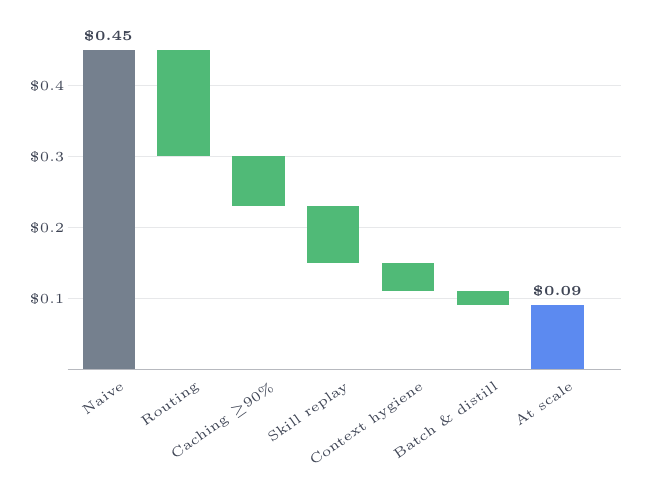
\begin{tikzpicture}[x=0.95cm, y=9cm]
  \draw[ink!30] (0,0) -- (7.4,0);
  \foreach \v in {0.1,0.2,0.3,0.4}{\draw[ink!10] (0,\v) -- (7.4,\v); \node[nb, anchor=east] at (0,\v) {\$\v};}
  % bars: name / bottom / top / colour
  \foreach \i/\n/\b/\t/\c in {0/Naive/0/0.45/slate, 1/Routing/0.30/0.45/leaf, 2/Caching $\ge$90\%/0.23/0.30/leaf,
                              3/Skill replay/0.15/0.23/leaf, 4/Context hygiene/0.11/0.15/leaf, 5/Batch \& distill/0.09/0.11/leaf, 6/At scale/0/0.09/accent}
  {
    \fill[\c!75] (\i+0.2,\b) rectangle (\i+0.9,\t);
    \node[nb, rotate=35, anchor=north east] at (\i+0.7,-0.01) {\n};
  }
  \node[nb, font=\tiny\bfseries] at (0.55,0.47) {\$0.45};
  \node[nb, font=\tiny\bfseries] at (6.55,0.11) {\$0.09};
\end{tikzpicture}
\end{diagram}
\column{0.45\textwidth}
\scriptsize
\begin{itemize}
  \item \textbf{Routing}: $\sim$60\% of calls to Haiku 4.5 / Sonnet 5 at low effort; frontier only for planning \& negotiation.
  \item \textbf{Caching}: frozen system prompt + tools + profile prefix; append-only transcripts.
  \item \textbf{Skill replay}: repeated merchant flows run as scripts; LLM only on drift.
  \item \textbf{Context hygiene}: clear old tool results, compaction, distilled observations instead of raw DOM.
  \item \textbf{Batch \& distill}: memory consolidation via Batch API (50\% off); small fine-tuned extractors.
  \item Per-user token budgets by plan tier; cost per \emph{completed} task is the KPI.
\end{itemize}
{\tiny\color{slate}Illustrative waterfall; measure on your own traffic.}
\end{columns}
\end{frame}

\begin{frame}{Browser, tools and voice at scale}
\begin{columns}[T]
\column{0.5\textwidth}
\small
\textbf{Browser fleet}
\begin{itemize}
  \item Kubernetes + Firecracker (or Kata / gVisor) microVM per session; warm pools per region; $\sim$1--2 GB RAM per session.
  \item Encrypted per-user browser profiles; secrets injected at the proxy, never shown to the model.
  \item Compile the top $\sim$500 merchant flows into scripts with self-healing selectors.
  \item Per-site circuit breakers \& rate limits; respect robots / ToS; prefer partner APIs and agentic-commerce protocols.
\end{itemize}
\column{0.5\textwidth}
\small
\textbf{Tool gateway}
\begin{itemize}
  \item MCP servers behind one gateway: per-user OAuth tokens, scopes, quotas, schema validation, idempotency, response caching.
  \item Integration SLOs and synthetic probes per vendor; auto-fallback to next rung of the ladder.
\end{itemize}
\textbf{Voice}
\begin{itemize}
  \item SIP trunks with regional capacity; realtime voice model streams; recordings stored per consent rules.
  \item Always disclose the AI; user can barge in from the app at any time.
\end{itemize}
\end{columns}
\end{frame}

\begin{frame}{Reliability and correctness}
\begin{columns}[T]
\column{0.5\textwidth}
\small
\textbf{Side effects}
\begin{itemize}
  \item Idempotency key on every side-effecting call, deduplicated at the tool gateway.
  \item Sagas with compensations: flight booked, hotel fails $\Rightarrow$ void ticket inside the void window.
  \item Money: issuer authorization bound to task id; daily reconciliation of orders $\leftrightarrow$ charges $\leftrightarrow$ tasks.
\end{itemize}
\textbf{Degradation}
\begin{itemize}
  \item LLM provider failover (Anthropic API $\leftrightarrow$ Bedrock $\leftrightarrow$ Vertex) behind the gateway.
  \item Non-urgent work queues instead of failing; ambient jobs shed first.
\end{itemize}
\column{0.5\textwidth}
\small
\textbf{SLOs}\\[2pt]
\scriptsize
\begin{tabular}{l r}
\toprule
API availability & 99.95\%\\
First streamed token & $<$ 1.5 s p95\\
Approval push delivered & $<$ 5 s p95\\
Task success (per vertical) & $\ge$ 90\%\\
Unauthorized spend & 0\\
Workflow durability & no lost tasks\\
\bottomrule
\end{tabular}\\[6pt]
\small
\textbf{Game days}: provider outage, merchant redesign, region fail-over, Temporal backlog surge, card-issuer outage.
\end{columns}
\end{frame}

\begin{frame}{Security, privacy and compliance}
\begin{columns}[T]
\column{0.33\textwidth}
\small
\textbf{Threats}
\begin{itemize}
  \item prompt injection via web \& email
  \item account takeover
  \item payment fraud
  \item data exfiltration
  \item malicious merchants / counter-agents
  \item misuse of agents at scale
\end{itemize}
\column{0.33\textwidth}
\small
\textbf{Controls}
\begin{itemize}
  \item dual-LLM containment + provenance
  \item egress allowlists; spend caps
  \item step-up auth for tier 3
  \item anomaly detection on agent actions
  \item red-team suites in CI; bug bounty
  \item per-user envelope encryption $\Rightarrow$ crypto-shredding on delete
\end{itemize}
\column{0.33\textwidth}
\small
\textbf{Compliance}
\begin{itemize}
  \item SOC 2 Type II, ISO 27001
  \item PCI DSS scope minimized via issuer tokens
  \item GDPR / CCPA: export, delete, EU residency
  \item EU AI Act transparency duties
  \item call-recording \& AI-voice rules (e.g.\ TCPA)
  \item no training on user data without opt-in
\end{itemize}
\end{columns}
\vfill
\small\textbf{User controls:} memory viewer / editor, full activity log with replays, per-merchant permissions, global kill switch.
\end{frame}

\begin{frame}{Evals and the quality flywheel}
\begin{columns}[c]
\column{0.52\textwidth}
\begin{diagram}
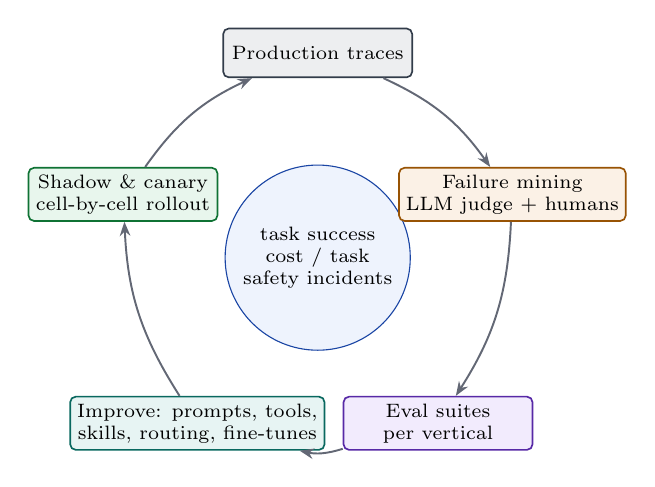
\begin{tikzpicture}
  \node[circle, draw=accent!70!black, fill=accent!8, font=\scriptsize, align=center, minimum size=2.0cm] (c) at (0,0)
     {task success\\cost / task\\safety incidents};
  \foreach \n/\a/\t/\col in {p/90/Production traces/slate, f/18/Failure mining\\LLM judge + humans/amber,
      e/-54/Eval suites\\per vertical/violet, i/-126/{Improve: prompts, tools,\\skills, routing, fine-tunes}/teal,
      r/162/Shadow \& canary\\cell-by-cell rollout/leaf}
    {\node[bx=\col, minimum width=2.4cm] (\n) at (\a:2.6) {\t};}
  \draw[ar] (p) to[bend left=15] (f); \draw[ar] (f) to[bend left=15] (e);
  \draw[ar] (e) to[bend left=15] (i); \draw[ar] (i) to[bend left=15] (r); \draw[ar] (r) to[bend left=15] (p);
\end{tikzpicture}
\end{diagram}
\column{0.48\textwidth}
\small
\begin{itemize}
  \item \textbf{Simulation environments}: recorded merchant sites (HAR replay), mock travel APIs, synthetic customer-service agents that negotiate back.
  \item \textbf{Adversarial pages} with injected instructions in every suite.
  \item Metrics per vertical: success, steps, cost, time, user edits to drafts, approvals denied.
  \item No prompt, model or skill change ships without passing the eval gate.
\end{itemize}
\end{columns}
\end{frame}

% =====================================================================
\section{Team, risks, takeaways}
% =====================================================================
\begin{frame}{Team shape as you scale}
\scriptsize
\renewcommand{\arraystretch}{1.35}
\begin{tabularx}{\linewidth}{>{\bfseries\raggedright\arraybackslash}p{2.3cm} X X X}
\toprule
 & Prototype (1k--5k) & Growth (100k) & Scale (1M+)\\
\midrule
Headcount & 4--6 engineers + PM / ops & 25--40 & 100+\\
Agent \& product & 2 full-stack agent engineers, 1 mobile / web & vertical pods: shopping, travel, service, ambient & + voice, A2A partnerships, personalization\\
Platform & 1 infra / security generalist & platform, data, browser fleet & SRE per region, cell platform, LLM gateway team\\
Quality \& safety & shared eval duty & evals team, trust \& safety & red team, fraud, compliance, privacy engineering\\
Operations & 2--4 HITL operators & HITL + support ($<$5\% of tasks) & support + escalations ($<$0.5\%)\\
Partnerships & -- & merchants, travel suppliers & payment networks, A2A / ACP ecosystems\\
\bottomrule
\end{tabularx}
\end{frame}

\begin{frame}{Risks and mitigations}
\scriptsize
\renewcommand{\arraystretch}{1.35}
\begin{tabularx}{\linewidth}{>{\bfseries\raggedright\arraybackslash}p{3.4cm} X}
\toprule
Risk & Mitigation\\
\midrule
Sites block agents / ToS conflicts & API-first, merchant partnerships, agentic-commerce protocols, user-present browsing, respectful rate limits\\
Prompt injection causes harmful action & dual-LLM containment, provenance-aware policy, approvals, per-task virtual-card caps\\
Cost per task outgrows revenue & routing, caching, skill replay, budgets per plan tier, cost-per-completed-task KPI\\
Wrong purchase / booking & verifier pass, explicit approval with summary, sagas \& easy undo, liability reserve / insurance\\
Regulation of AI calls \& agents & AI disclosure, consent capture, jurisdiction-aware rules engine, audit trail\\
User trust \& privacy & transparent, editable memory; encryption; no training without opt-in; data residency\\
Model or provider outage & multi-provider gateway, graceful degradation, queued non-urgent work\\
\bottomrule
\end{tabularx}
\end{frame}

\begin{frame}{Key takeaways}
\begin{enumerate}
  \item A personal agent is a \textbf{durable, memory-rich workflow system} with an LLM inside -- not a chatbot with tools.
  \item Start with the \textbf{composite}: orchestrator + specialists on durable workflows, MCP-first tools, browser fallback, policy engine, human-in-the-loop.
  \item \textbf{Bound the blast radius} before adding autonomy: permission tiers, virtual cards, quarantined readers, audit.
  \item The prototype stack is \textbf{boring on purpose}: FastAPI, Temporal, Postgres + pgvector, hosted browsers, Claude API, Stripe Issuing.
  \item Scaling to millions is mostly \textbf{cost-down and blast-radius control}: routing, caching, skill replay, cells, multi-provider capacity.
  \item The moat is \textbf{memory + evals}: knowing the user and proving the agent gets things right.
\end{enumerate}
\end{frame}

\end{document}
